\section*{Learning Objectives}

By the end of this chapter, students should be able to:
\begin{itemize}
    \item Define improper integrals and understand their significance within the context of calculus.
    \item Identify integrals that may pose difficulties due to their unbounded nature or the behavior of the function being integrated.
    \item  Answer the pressing question: can an integral be doubly improper?
    \item Explore the applications of improper integrals, emphasizing their practical importance in Statistics and Probability.
\end{itemize}

\section*{Outcomes}

Upon successful completion of this chapter, students will:
\begin{itemize}
    \item Master the technique of integrating over unbounded domains using limits.
    \item Learn to manage and integrate functions with singularities or discontinuities by applying limits to circumvent infinite behavior at finite points, thus handling vertical asymptotes effectively.
    \item Gain a comprehensive understanding of the analytical methods for solving improper integrals, employing antiderivatives to facilitate calculation.
    \item Acquire skills in applying numerical methods, specifically Julia's \texttt{QuadGK}, for evaluating improper integrals, particularly when analytical solutions are challenging to obtain.
    \item Delve into two probability theory examples that utilize improper integrals, reinforcing the concept’s application in real-world scenarios and theoretical studies.
\end{itemize}




\newpage




\section{Introduction}

What a name, right? \textbf{Improper?} In short, the term ``improper integral'' serves as a descriptive label to indicate that the integral in question deviates from the standard conditions that apply to definite integrals, and hence, extra caution is advised. The word ``improper'' in this context doesn't imply that there's something wrong or less valid about the integrals we study in this Chapter. Rather, it indicates that they don't fit within the framework of standard definite integrals and require special techniques for their evaluation. These techniques involve taking limits, as the interval of integration or the function itself is unbounded. The terminology likely originated to help mathematicians categorize and study different types of integrals, especially as the field of real analysis began to formalize concepts related to integration. \textcolor{red}{\bf The term helps to signal that additional care or ``alternative methods'' may be needed to evaluate the integral.}



\section{Type-I Improper Integrals: Unbounded Limits of Integration}

We first look at cases where the integrand, $f$, is piecewise continuous, and hence, for any closed and bounded interval $[a, b]$, the definite integral $\int_a^b f(x) \, dx$ exists and is finite. We are interested in what happens as one or more of the limits of integration is unbounded, that is, $\int_a^\infty f(x) \, dx$,  $\int_{-\infty}^b f(x) \, dx$, and a bit later,  $\int_{-\infty}^\infty f(x) \, dx$. So that we can understand what the issues are, let's look at a few examples first.
\begin{itemize}
    \item Let $f:[0, \infty) \to \real$ by $f(x) = e^{-x}$. Then, $\int_0^b f(x) \, dx = -e^{-x}~\bigg|_0^b = 1 - e^{-b}$. Hence, $\displaystyle \lim_{b \to \infty}  \int_0^b f(x) \, dx = \lim_{b \to \infty} \left(1 - e^{-b}\right) = 1.0$. Because the value of the integral is finite, we say it is \textbf{convergent}.
    \item Let $f:[0, \infty) \to \real$ by $f(x) = 1$. Then, $\int_0^b f(x) \, dx = b$. Hence, $\displaystyle \lim_{b \to \infty} \int_0^b f(x) \, dx = \infty$. Because the value of the integral is unbounded, we say it is \textbf{divergent}.
    \item Let $f:(-\infty, 0] \to \real$ by $f(x) = \cos(x)$. Then, $\int_a^0 f(x) \, dx = \sin(x)~\bigg|_{a}^0 = -\sin(a)$. Hence, $\displaystyle \lim_{a \to -\infty}  \int_a^0 f(x) \, dx = \lim_{a \to -\infty} -\sin(a)$ is \textbf{undefined}.
\end{itemize}

\bigskip
The following definitions are based on the previous three examples. 
\bigskip

\begin{tcolorbox}[colback=mylightblue, title = {\bf Unbounded Upper or Lower Limit: Take 1}, breakable]
\begin{definition}
\label{def:unboundedLimitsOfIntegration}
Suppose that  $f:[a, \infty) \to  \real$ is a real-valued function, and for all $b>a$ (finite), $\int_a^b f(x) \, dx$ exists and is finite\footnote{If $f:[a, \infty) \to  \real$ is piecewise continuous, then this condition is met.}. Then,
\begin{equation}
    \label{eq:unboundedUpperLimit}
    \int_a^\infty f(x) \, dx := \lim_{b \to \infty} \int_a^b f(x) \, dx,
\end{equation}
if the limit exists. The integral is \textbf{undefined} otherwise. If the limit exists but is unbounded (i.e., equals $\pm \infty$), then we say the integral is \textbf{divergent}, while if the limit exists and is finite, we say the integral is \textbf{convergent}.\\

Similarly, suppose that  $f:(-\infty, b] \to  \real$ is a real-valued function, and for all $a<b$ (finite), $\int_a^b f(x) \, dx$ exists and is finite\footnote{If $f:(-\infty, b] \to  \real$ is piecewise continuous, then this condition is met.}. Then,
\begin{equation}
    \label{eq:unboundedLowerLimit}
    \int_{-\infty}^b f(x) \, dx := \lim_{a \to -\infty} \int_a^b f(x) \, dx,
\end{equation}
if the limit exists. The integral is undefined otherwise. If the limit exists but is unbounded, (i.e., equals $\pm \infty$), then we say the integral is \textbf{divergent}, while if the limit exists and is finite, we say the integral is \textbf{convergent}.\\

\end{definition}

\end{tcolorbox}


\bigskip

\begin{example} 
\label{ex:SingleSidedImproperIntegrals}
Determine values, if possible, for the following improper integrals. You may wish to use the antiderivatives in Table.~\ref{tab:CommonFunctionsAndTheirAntiderivatives} and Table.~\ref{tab:CommonFunctionsAndTheirAntiderivativesWithScalingShift} because the integrands are very standard functions.
 \begin{enumerate}
\renewcommand{\labelenumi}{(\alph{enumi})}
\setlength{\itemsep}{.2cm}
    \item $\int_0 ^\infty x \, dx$.

    \item $\int_0 ^\infty e^{-x} \, dx$.

    
    \item $\int_{-\infty}^0 e^{-x} \, dx$.

    \item $\int_{-\infty} ^0 \sin(x) \, dx$.

\end{enumerate}
    
\end{example}

\textbf{Solutions:} 

 \begin{enumerate}
\renewcommand{\labelenumi}{(\alph{enumi})}
\setlength{\itemsep}{.2cm}
    \item \Ans \quad $\int_0 ^\infty x \, dx = \infty$.\\

    From Table.~\ref{tab:CommonFunctionsAndTheirAntiderivatives}, $\int_0^b x \, dx = \frac{1}{2} x^2~ \bigg|_0^b =  \frac{b^2}{2}$. Hence,  $\int_0 ^\infty x \, dx :=\displaystyle \lim_{b \to \infty} \int_0^b x \, dx = \lim_{b \to \infty} \frac{1}{2} b^2 = \infty$.

    \item \Ans \quad $\int_0 ^\infty e^{-x} \, dx = 1$.\\

    From Table.~\ref{tab:CommonFunctionsAndTheirAntiderivativesWithScalingShift}, $\int_0 ^b e^{-x} \, dx = - e^{-x}~\bigg|_0^b =  -\left( e^{-b} - 1 \right) = 1 - e^{-b}$. Hence, $\int_0 ^\infty e^{-x} \, dx :=\displaystyle \lim_{b \to \infty} \int_0^b e^{-x} \, dx = \lim_{b \to \infty} 1 - e^{-b} = 1$. We can also use quadGK:

\begin{lstlisting}[language=Julia,style=mystyle]
using QuadGK

f(x) = exp(-x)
Data = Array{Float64}(undef, 0, 3)
#
for b=0:2:30
    value, error = quadgk(f, 0, b)
    Data = [Data; b value error]
end
Data
\end{lstlisting}
\textbf{Output} 
\begin{verbatim}
16×3 Matrix{Float64}:
  0.0  0.0       0.0
  2.0  0.864665  7.77156e-16
  4.0  0.981684  1.00392e-11
  6.0  0.997521  1.74719e-9
  8.0  0.999665  1.02231e-11
 10.0  0.999955  1.804e-10
 12.0  0.999994  1.75152e-9
 14.0  0.999999  1.12599e-8
 16.0  1.0       2.81922e-11
 18.0  1.0       7.20663e-11
 20.0  1.0       2.09573e-10
 22.0  1.0       6.26783e-10
 24.0  1.0       1.77795e-9
 26.0  1.0       4.65932e-9
 28.0  1.0       1.1276e-8
 30.0  1.0       2.97104e-11
\end{verbatim}
The improper integral converges very quickly to one. 

  \item \Ans \quad $\int_{-\infty}^0 e^{-x} \, dx = \infty$.\\

    From Table.~\ref{tab:CommonFunctionsAndTheirAntiderivativesWithScalingShift}, $\int_{a}^0 e^{-x} \, dx = - \left( 1 - e^{-a} \right) = e^{-a} -1$. Hence, $\int_{-\infty}^0 e^{-x} \, dx :=\displaystyle \lim_{a \to -\infty} \int_a^0 e^{-x} \, dx = \lim_{a \to -\infty} e^{-a} -1 = \infty$.
    

    \item \Ans \quad $\int_{-\infty} ^0 \sin(x) \, dx$ is undefined because the limit does not exist.\\

    \textbf{Intuition:} We know that $\sin(x)$ oscillates between plus and minus one. Moreover, $\sin(x+\pi) = -\sin(x)$, and hence, the integral over $2 \pi$-interval $[k\pi, (k+2)\pi]$ is equal to zero. Therefore, we do not expect the integral to converge. But we check it out anyway, just to confirm our intuition. \\

    We can use antiderivatives for an analytical approach: $\int_{a} ^0 \sin(x) \, dx = -\cos(x)~\bigg|_a^0 = \cos(a)$. Hence, $\int_{-\infty} ^0 \sin(x) \, dx = \displaystyle \lim_{a \to \infty } \cos(a)$, which does not exist.\\

    We can also see via numerical integration that something is not right!     
\begin{lstlisting}[language=Julia,style=mystyle]
using QuadGK, Plots, LaTeXStrings
    
f(x) = sin(x)
Data = Array{Float64}(undef, 0, 3)
#
a0=-30*pi
for a=a0:-.01:(a0-6pi)
    value, error = quadgk(f, a, 0)
    Data = [Data; a value error]
end
p1 = plot(Data[:,1], Data[:,2], linewidth=4, color=:blue, label=false)
plot!(xlabel=L"$a$", ylabel=L"$y= \int_a^0 \sin(x) \, dx$") 

display(p1)
\end{lstlisting}
\textbf{Output} 

   \begin{center}
    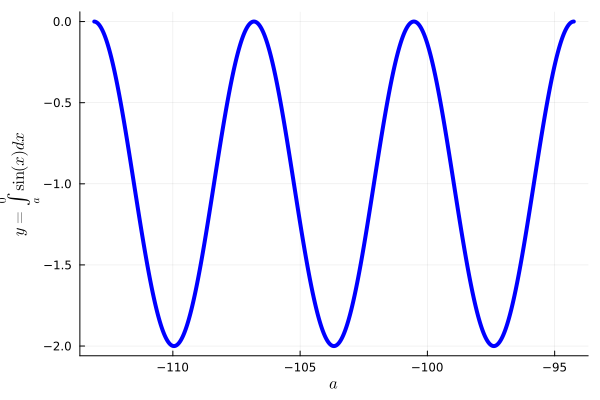
\includegraphics[width=0.45\columnwidth]{graphics/Chap04/ImproperIntegralSine.png}
    \end{center}

   
\end{enumerate}

    \Qed



\bigskip

\emstat{ Functions defined on $(-\infty, \infty)$ pose an extra layer of difficulty. To see why, consider, $f:\real \to \real$ by $f(x) = 4x^3$. Then, $\int_a^b f(x) \, dx = x^4~\bigg|_{a}^b = b^4 - a^4$. Hence, $\displaystyle \lim_{a \to -\infty}  \int_a^b f(x) \, dx = \lim_{a \to -\infty} b^4-a^4 = -\infty$. But if we evaluate  $\displaystyle \lim_{b \to \infty}  \int_a^b f(x) \, dx = \lim_{b \to \infty} b^4-a^4 = \infty$. So what value should we assign to $\int_{-\infty}^\infty f(x) \, dx$? }

\bigskip
\begin{funColor}{A Word of Caution for Doubly-infinite Integrals}{DoubleInfinity}

In general, $\int_{-\infty}^\infty f(x) \, dx \neq \displaystyle \lim_{c \to \infty} \int_{-c}^c f(x) \, dx$. \textcolor{blue}{\bf You must compute the two limits}, $\RED \displaystyle \lim_{c \to \infty} \int_{-c}^0 f(x) \, dx$ \textcolor{blue}{\bf and} $\RED \displaystyle \lim_{c \to \infty} \int_{0}^c f(x) \, dx$, \textcolor{red}{\bf SEPARATELY!!!}. Why? Consider
    $$\int_{-c}^c x \, dx.$$
    Then, as illustrated in the figure below, the magnitude of the negative area is exactly equal to the positive area, and hence for any interval $[-c, c]$ that is symmetric about the origin, $\int_{-c}^c x \, dx=0.0$, i.e., the areas cancel out, exactly. However, $\int_{-\infty}^0 x \, dx = -\infty$ and $\int_0^{\infty} x \, dx = +\infty$, which do NOT cancel out; the their sum is undefined. Moreover, if we computed $\displaystyle \lim_{c \to \infty}\int_{-c}^{c+1} x \, dx$, we'd obtain positive infinity, and if we computed  $\displaystyle \lim_{c \to \infty}\int_{-c^3}^{c^2} x \, dx$, we'd obtain negative infinity. In other words, the limit changes if we advance more quickly in one direction than the other. \textcolor{blue}{\bf We avoid this problem by assessing the two limits separately and then analyzing whether their sum makes sense (or not). The sum will make sense except when both limits are unbounded and have opposite signs, giving rise to the notorious, ``$\bm{\infty - \infty}$''.}

      \begin{center}
    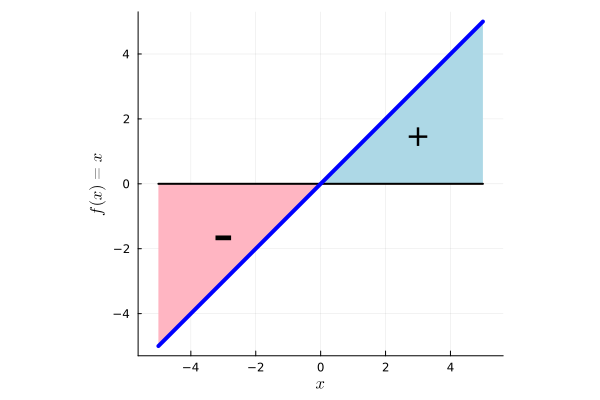
\includegraphics[width=0.45\columnwidth]{graphics/Chap04/IntegralOfmonomialXSymmetricInterval.png}
    \end{center}

\textbf{Note:} The symmetric limit, $\displaystyle \lim_{c \to \infty} \int_{-c}^c f(x) \, dx$, has a name: the \textbf{Cauchy Principal Value}; see \href{https://en.wikipedia.org/wiki/Cauchy_principal_value}{Wikipedia} for more information.
\end{funColor}

\bigskip

\begin{tcolorbox}[colback=mylightblue, title = {\bf Unbounded Upper and Lower Limit: Take 2}, breakable]
\begin{definition}
\label{def:unboundedLimitsOfIntegrationTake2}

Suppose that  $f:(-\infty, \infty) \to  \real$ is a real-valued function, and for all $a<b$ (both finite), $\int_a^b f(x) \, dx$ exists and is finite\footnote{If $f:(-\infty, \infty) \to  \real$ is piecewise continuous, then this condition is met.}. Then,
\begin{equation}
    \label{eq:unboundedLowerUpperLimit}
    \int_{-\infty}^\infty f(x) \, dx := \lim_{a \to -\infty} \int_a^0 f(x) \, dx + \lim_{b \to \infty} \int_0^b f(x) \, dx,
\end{equation}
if both limits exist and are finite (i.e., both integrals are convergent). If one of the limits is undefined, then the integral is undefined. If both limits exist but at least one is unbounded (i.e, $\pm \infty$), more care is required to avoid $\infty - \infty$. Hence,
\begin{itemize}
    \item if one limit is unbounded while the other is finite, then the value of the unbounded limit is the value of the integral;
    \item if both limits are unbounded and have the same sign, then the common value of the unbounded limits is the value of the integral; and as was said above,
    \item if one limit equals $+\infty$ and the other $-\infty$, then the integral is \textbf{undefined}.
\end{itemize} 
\end{definition}

\end{tcolorbox}


\bigskip

\begin{example} Determine values, if possible, for the following improper integrals. You may wish to use the antiderivatives in Table.~\ref{tab:CommonFunctionsAndTheirAntiderivatives} and Table.~\ref{tab:CommonFunctionsAndTheirAntiderivativesWithScalingShift} because the integrands are very standard functions.
 \begin{enumerate}
\renewcommand{\labelenumi}{(\alph{enumi})}
\setlength{\itemsep}{.2cm}

    \item $\int_{-\infty}^\infty x \, dx$.

    \item $\int_{-\infty}^\infty x^2 \, dx$.


    \item $\int_{-\infty}^\infty e^{-x} \, dx$.

\end{enumerate}
    
\end{example}

\textbf{Solutions:} 

 \begin{enumerate}
\renewcommand{\labelenumi}{(\alph{enumi})}
\setlength{\itemsep}{.2cm}
   

    \item \Ans \quad $\int_{-\infty}^\infty x \, dx$ is undefined because we have ``$-\infty + \infty$''.\\

      From Table.~\ref{tab:CommonFunctionsAndTheirAntiderivatives}, $\int_a^0x \, dx = -\frac{1}{2} a^2$. Hence,  $\int_0 ^\infty x \, dx :=\displaystyle \lim_{a \to -\infty} \int_a^0 x \, dx = \lim_{a \to -\infty} -\frac{1}{2} a^2 = -\infty$. From part (a) of this Example, $\int_0 ^\infty x \, dx = \infty$. Hence, $\int_{-\infty} ^\infty x \, dx = -\infty + \infty =$ undefined.

    \item \Ans \quad $\int_{-\infty}^\infty x^2 \, dx = \infty$ because the two limits share the same sign and at least one is unbounded.\\

    From Table.~\ref{tab:CommonFunctionsAndTheirAntiderivatives}, $\int_a^0 x^2 \, dx = -\frac{1}{3} a^3$. Hence,  $\int_{-\infty} ^0 x^2 \, dx :=\displaystyle \lim_{a \to -\infty} \int_a^0 x^2 \, dx = \lim_{a \to -\infty} -\frac{1}{3} a^3 = +\infty$. Similarly,  $\int_0^b x^2 \, dx = \frac{1}{3} b^3$. Hence,  $\int_0 ^\infty x^2 \, dx :=\displaystyle \lim_{b \to \infty} \int_0^b x^2 \, dx = \lim_{b \to \infty} \frac{1}{3} a^3 = \infty$. Therefore, $\int_{-\infty} ^\infty x^2 \, dx  = \infty + \infty = \infty$.

  

    \item \Ans \quad $\int_{-\infty}^\infty e^{-x} \, dx = \infty$ because one limit is bounded and the other is unbounded.\\

    In Example~\ref{ex:SingleSidedImproperIntegrals}, we computed each limit separately. The rest is left to the learner. \Qed

\end{enumerate}

\vspace*{0.5cm} 

\begin{figure}[ht]%
\centering    
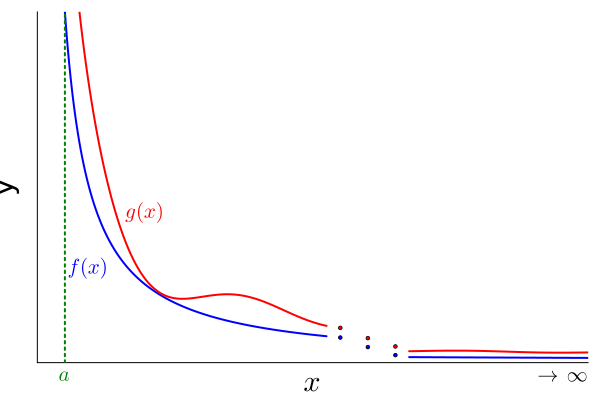
\includegraphics[width=0.6\columnwidth]{graphics/Chap08/ComparisonTest.png}%
    \caption[]{\textbf{Comparison Test:} Suppose that $f:[a, \infty) \to [0, \infty)$ and $g:[a, \infty) \to [0, \infty)$ are piecewise continuous functions so that their Riemann Integrals exist and are finite for any bounded interval $[a, b]$. When are they finite on $[a, \infty)$? In the plot, we observe that $f(x) \le g(x)$ for all $x \in [a, \infty)$, and hence, on one hand, if the area under $g$ is finite, so must be the area under $f$, and on the other hand, if the area under $f$ is unbounded, so must be the area under $g$. \textcolor{blue}{\bf These simple observations are the heart of the comparison test.}}
    \label{fig:ComparisionTest}
\end{figure}


\bigskip

\subsection{Comparision Test}
\label{sec:ComparisonTest}
 It would be nice to have some rules of thumb for knowing when an improper integral should exist and be finite and when it is likely to be unbounded. Figure~\ref{fig:ComparisionTest} shows that by comparing one function against another function's KNOWN behavior, we can make conclusions about an integral of the form $\int_a^\infty f(x) \, dx$ by comparing it to another integral $\int_a^\infty g(x) \, dx$. Indeed, if $0\le f(x) \le g(x)$, then 
 \begin{itemize}
     \item $\int_a^\infty g(x) \, dx < \infty \implies \int_a^\infty f(x) \, dx < \infty $, and 
     \item $\int_a^\infty f(x) \, dx =\infty \implies \int_a^\infty g(x) \, dx = \infty $. 
 \end{itemize}
 
 That is interesting, but what are some relevant comparison functions to use? We dig into our antiderivative bag of easy integrals and make some observations.
\begin{enumerate}
\renewcommand{\labelenumi}{(\alph{enumi})}
\setlength{\itemsep}{.2cm}

    \item For all $p>1$, $\int_1^b \frac{1}{x^p} \, dx = \int_1^b x^{-p} \, dx = \frac{x^{1-p}}{1-p}~\bigg|_1^b = \frac{b^{1-p}}{1-p} - \frac{1}{1-p} = \frac{1}{1-p} \cdot \left(\frac{1}{b^{p-1}} -1 \right) $. 
    For $p>1$, it follows that $p-1 >0$, and hence  ${\displaystyle \lim_{b \to \infty}} \frac{1}{b^{p-1}} = 0$. Therefore,  $\int_1^\infty \frac{1}{x^p} \, dx  = \frac{-1}{1-p} = \frac{1}{p-1}< \infty$.
    

        
    \item $\int_1^b \frac{1}{x} \, dx = \ln(x)~\bigg|_1^b = \ln(b)$ and hence $\int_1^\infty \frac{1}{x} \, dx = \displaystyle \lim_{b \to \infty} \ln(b) = \infty$. This makes sense because as $p \to 1^+$ in part (a), we see that the value of the integral, $\frac{1}{p-1}$, diverges to infinity.
    
    \item For all $0 \le p < 1$,  $\int_1^b \frac{1}{x^p} \, dx = \int_1^b x^{-p} \, dx = \frac{x^{1-p}}{1-p}~\bigg|_1^b = \frac{b^{1-p}}{1-p} - \frac{1}{1-p} = \frac{1}{1-p} \cdot \left(b^{1-p} -1 \right) $.  For $p<1$, it follows that $1-p >0$, and hence  ${\displaystyle \lim_{b \to \infty}} ~b^{1-p} = \infty$. Therefore,  $\int_1^\infty \frac{1}{x^p} \, dx  = \infty$.

\end{enumerate}

The above analysis says that $\frac{1}{x}$ is a  ``line of demarcation'' between an improper integral of $\frac{1}{x^p}$ being unbounded (for $0\le p \le 1$) and being finite (for $p>1$). Hence, we can use $\frac{1}{x^p}$ in the \textbf{Comparison Test} illustrated in Fig.~\ref{fig:ComparisionTest} and stated more formally below.

\bigskip
Recall that for any $a < b$ finite and any piecewise continuous function $f:[a, b] \to \real$, the Riemann integral, $\int_a^b f(x) \, dx$, exists and is finite. Hence, an improper integral, e.g., $\int_a^\infty f(x) \, dx$, is finite (or is infinite, or does not exist) if, and only if, for any $c\ge a$ finite, $\int_c^\infty f(x) \, dx$, is finite (or is infinite, or does not exist), respectively. In other words, because 
$\int_a^c f(x) \, dx$ is guaranteed to be finite, we can ignore it when trying to understand if the $\int_a^\infty f(x) \, dx$, is convergent or not. Why is this a helpful observation? We;ll see in examples that by choosing $c$ sufficiently large, we can sometimes use ``asymptotic reasoning'' to form more easily an upper bound or a lower bound on $f:[c, \infty) \to \real$ than we can for $f:[a, \infty) \to \real$.
\bigskip

\begin{propColor}{Comparision Test}{ComparisionTest}
    Consider a \textbf{non-negative piecewise continuous} function $f:[0, \infty) \to [0, \infty)$ and a second non-negative piecewise continuous function, $g:[c, \infty) \to [0, \infty)$, where $c\ge 0$. Then the following are true:

    \begin{enumerate}
\renewcommand{\labelenumi}{(\alph{enumi})}
\setlength{\itemsep}{.2cm}
    \item \textbf{Test for a convergent (aka, finite) improper integral:}
    \begin{itemize}
        \item Suppose that for all $x \ge c$, $f(x) \le g(x)$ (one says that $f$ is upper bounded by $g$ on $[c, \infty)$, or $f$ is eventually upper bounded by $g$), and 
        \item  $\int_c^\infty g(x) \, dx$ exists and is finite. 
    \end{itemize}
    Then $\int_0^\infty f(x) \, dx$ exists and is finite. (In other words, $f$ being eventually upper bounded by a function with a finite improper integral ensures that its improper integral is also finite).
    \item \textbf{Test for a divergent (aka, unbounded) improper integral:}
      \begin{itemize}
        \item Suppose that for all $x \ge c$, $g(x) \le f(x)$ (one says that $f$ is lower bounded by $g$ on $[c, \infty)$, or $f$ is eventually lower bounded by $g$), and 
        \item  $\int_c^\infty g(x) \, dx$ exists and is infinite. 
    \end{itemize}
    Then $\int_0^\infty f(x) \, dx$ exists and is infinite. (In other words, $f$ being lower bounded by a function with an unbounded improper integral implies that its improper integral is also unbounded.)
\end{enumerate}   

\textbf{Note:} We leave the cases for functions defined on $(-\infty, 0]$ to the learner. \\

\textbf{Note:} The second part of  Fig.~\ref{fig:ComparisionTest}  shows that if a piecewise continuous function  $f:[0, \infty) \to \real$ takes on both positive and negative values, then useful information is obtained by applying the comparison test to the function's absolute value.    
\end{propColor}

\bigskip

\begin{example} 
\label{ex:ComparisonTest01}
Use the Comparison Test to determine which of the following improper integrals are convergent or divergent.
\begin{enumerate}
\renewcommand{\labelenumi}{(\alph{enumi})}
\setlength{\itemsep}{.2cm}
    \item $\int_0^\infty \frac{1}{x^2 + 1} \, dx$, where we note that the denominator has no real roots, and hence $\frac{1}{x^2 + 1}$ is finite for all $x\in \real$.
    \item $\int_0^\infty \frac{\sin(x)}{x^2 + 1} \, dx$.
    \item $\int_0^\infty \frac{x}{x^2 + 1} \, dx$.
    \item $\int_0^\infty \frac{x^3 + 4}{x^5 - 3x +21} \, dx$, where the denominator has one real root at $ x \approx -1.93017$ and four complex roots.
    \item $\int_0^\infty \frac{x + e^{-x}}{x^2 + 1} \, dx$.
    \item $\int_0^\infty e^{-x} \cdot\frac{x^4 + 111}{x^2 + 1} \, dx$.
 \end{enumerate}    
\end{example}
\textbf{Solutions:}

\begin{enumerate}
\renewcommand{\labelenumi}{(\alph{enumi})}
\setlength{\itemsep}{.2cm}
    \item $\int_0^\infty \frac{1}{x^2 + 1} \, dx$ is convergent. Let $f(x) := \frac{1}{x^2 + 1} = \frac{\frac{1}{x^2}}{1 + \frac{1}{x^2}}$, where we divided the numerator and denominator by $x^2$. Next, we note that $1 + \frac{1}{x^2} > 1$ for all $x\ge 0$. Hence, $f(x) \le g(x) := \frac{1}{x^2}$ for all $x\ge 0$. We know that $ \int_0^\infty g(x) \, dx$ is convergent, and therefore, so is  $\int_0^\infty f(x) \, dx$.\\

    Note: For this integrand, we know that $\atan(x)$ is an antiderivative of  $\frac{1}{x^2 + 1}$. Hence, $\int_0^\infty \frac{1}{x^2 + 1} \, dx = \atan(x)~\bigg|_0^\infty =\frac{\pi}{2}$.

 \item $\int_0^\infty \frac{\sin(x)}{x^2 + 1} \, dx$ is convergent. Because $|\sin(x)| \le 1$, we have that $\bigg| \frac{\sin(x)}{x^2 + 1}\bigg| \le \frac{1}{x^2 + 1}$. From (a), we know that $\int_0^\infty \frac{1}{x^2 + 1} \, dx$ is convergent. Hence, $\int_0^\infty \frac{\sin(x)}{x^2 + 1} \, dx$ is also convergent.

 
\item $\int_0^\infty \frac{x}{x^2 + 1} \, dx$ is divergent. Did you see that coming? Let $f(x):=\frac{x}{x^2 + 1} =  \frac{\frac{1}{x}}{1 + \frac{1}{x^2}}$, where we divided the numerator and denominator by $x^2$. Next, we note that $1 + \frac{1}{x^2} \le 2$ for all $x\ge 0$.  Hence, $f(x) \ge g(x) := \frac{1}{2} \cdot \frac{1}{x}$ for all $x\ge 0$. We know that $ \int_0^\infty g(x) \, dx$ is divergent, and therefore, so is  $\int_0^\infty f(x) \, dx$.\\ 

\item $\int_0^\infty \frac{x^3 + 4}{x^5 - 3x +21} \, dx$ is convergent. First of all, why was it important to note that the denominator has one real root at $ x \approx -1.93017$ and four complex roots? Because there are no positive real roots, the denominator does not vanish for any $x \ge 0$, and hence, we are never diving by zero. Therefore, $f(x) := \frac{x^3 + 4}{x^5 - 3x +21}$ is a continuous function on $[0, \infty)$. \\

Now, we turn to checking if the integral is convergent or divergent. We divide the numerator and denominator by $x^5$, giving us, 
$$ f(x) = \frac{\frac{1}{x^2} + \frac{4}{x^5}}{1 - \frac{3}{x^4} + \frac{21}{x^5}}.$$
For all $x\ge 10$, ${\rm den}(x):= 1 - \frac{3}{x^4} + \frac{21}{x^5} \ge 1  - \frac{3}{10^4} + \frac{21}{10^5} =\ge 0.99$. Using this bound, we have that for all $x\ge 10$
$$f(x) = \frac{\frac{1}{x^2} + \frac{4}{x^5}}{1 - \frac{3}{x^4} + \frac{21}{x^5}} \le \frac{\frac{1}{x^2} + \frac{4}{x^5}}{0.99}.$$
Because $\frac{1}{x^2}$ and $\frac{1}{x^5}$ are both convergent, we deduce that  $\int_{10}^\infty \frac{x^3 + 4}{x^5 - 3x +21} \, dx$ is convergent, which then implies that $\int_0^\infty \frac{x^3 + 4}{x^5 - 3x +21} \, dx$ is convergent.

    \item $\int_0^\infty \frac{x + e^{-x}}{x^2 + 1} \, dx$ is divergent. We write the integral as 
    $$\int_0^\infty \frac{x + e^{-x}}{x^2 + 1} \, dx = \int_0^\infty \frac{x }{x^2 + 1} \, dx + \int_0^\infty \frac{e^{-x}}{x^2 + 1} \, dx.$$

    Because $e^{-x} \le 1$ for all $x \ge 0$,  $\int_0^\infty \frac{e^{-x}}{x^2 + 1} \, dx \le \int_0^\infty \frac{1}{x^2 + 1} \, dx$, which we know to be convergent. However, we already know $\int_0^\infty \frac{x }{x^2 + 1} \, dx$ is divergent. Because the sum of something unbounded and something bounded is unbounded, we conclude that the overall integral is divergent. If both had been divergent, we would have to check that we are not committing the crime of $\infty - \infty$! Clear enough?

   \item $\int_0^\infty e^{-x} \cdot\frac{x^4 + 111}{x^2 + 1} \, dx$ is convergent. The intuition is that decaying exponentials crush exploding polynomials, which we established in Proposition ~\ref{thm:ExponentialsAreFast} and Corollary~\ref{thm:ExponentialsDecayFast}. But we can do better and show this analytically. Ignorign th exponential for a moment and focusing on the rational function, 
  \begin{align*}
      \frac{x^4 + 111}{x^2 + 1} &= \frac{x^4}{x^2} \,  \frac{1 + \frac{111}{x^4}}{1 + \frac{1}{x^2}} ~~(\text{factor our highest power from numerator and denominator})\\[1em] 
      &\le x^2 \frac{1 + \frac{111}{x^4}}{1}  ~~(\text{lower bound on the denominator holds for all}~~ x\ge 0)\\[1em] 
      &\le 2x^2  ~~(\text{for all}~~x>\sqrt[4]{111}).
  \end{align*} 
 This yields,  
  $\int_{10}^\infty e^{-x} \cdot\frac{x^4 + 111}{x^2 + 1} \, dx \le \int_{10}^\infty 2 \, x^2 e^{-x} \, dx = -2x^2e^{-x} + 4xe^{-x} - 4e^{-x} \Bigg|_{10}^\infty \approx 0.003723 $,
   and because   $\int_0^{10} e^{-x} \cdot\frac{x^4 + 111}{x^2 + 1} \, dx$ is finite, the overall integral is then finite, in other words, convergent.
 \end{enumerate}
\Qed

\bigskip 

Way back in Proposition ~\ref{thm:ExponentialsAreFast} and Corollary~\ref{thm:ExponentialsDecayFast}, we learned that exponentials dominate polynomials and rational functions when taking limits as $x \to \infty$. You may suspect that the presence of a decaying or exploding exponential in an integrand affects whether the integral is convergent or not, and you would be right! 

\begin{figure}[htb]%
\centering
\hfill
\subfloat[]{%
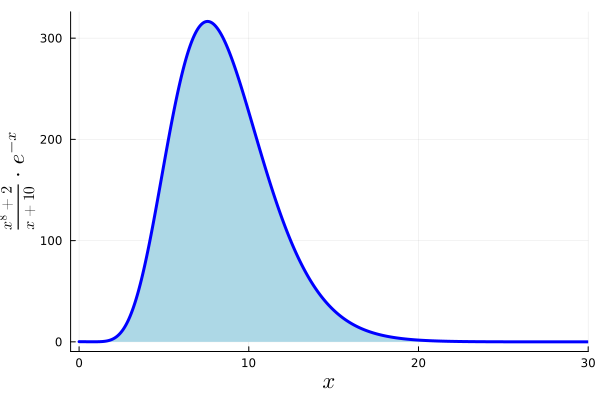
\includegraphics[width=0.45\columnwidth]{graphics/Chap08/ConvergentDivergentFamiliesImproperIntegrals.png}}%
\hfill%
\subfloat[]{%
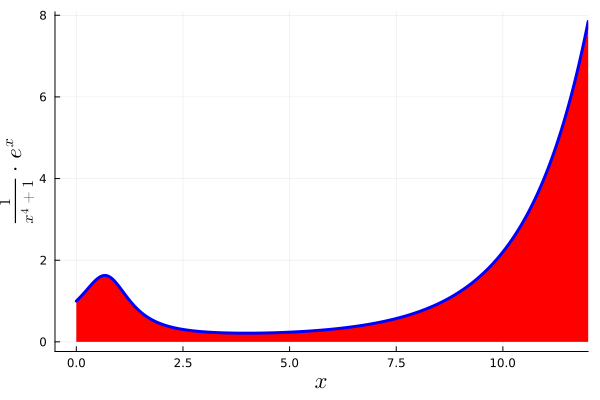
\includegraphics[width=0.45\columnwidth]{graphics/Chap08/ConvergentDivergentFamiliesImproperIntegralsV02.png}}%
\hspace*{1cm}
    \caption[]{\textbf{When Present, Exponentials Determine Convergence of Improper Integrals:} (a) Shows an exploding rational function, $\frac{x^8+2}{x + 10}$, times a decaying exponential, $e^{-x}$. The area under the function is finite. (b) Shows a decaying rational function, $\frac{1}{x^4 + 1}$, times an exploding exponential, $e^x$. The area under the function is infinite.}
    \label{fig:ConvergentDivergentFamiliesImproperIntegrals}
\end{figure}

\bigskip

\begin{propColor}{Families of Convergent and Divergent Improper Integrals: Take 1}{Type1GeneralFamily}

For all real numbers $\alpha>0$ and integers $k \ge 0$, the following hold:

\begin{enumerate}
\renewcommand{\labelenumi}{(\alph{enumi})}
\setlength{\itemsep}{.2cm}
    \item $\int_0^\infty x^k \cdot e^{-\alpha x} dx$ is convergent.

    \item  $\int_0^\infty  \frac{1}{x^k} \cdot e^{\alpha x} \, dx$ is divergent.

     \end{enumerate}
\bigskip
    
\end{propColor}

\textbf{Proof:} Part (a): For $k\ge 0$, define  $\gamma(k):= \int_0^\infty x^k \cdot e^{-\alpha x} dx$. We prove by induction that $\gamma(k) < \infty$ for all $k \ge 0$. The base case is easy, because $\gamma(0) = \int_0^\infty e^{-\alpha x} dx = \frac{1}{\alpha}$. Next, we assume the result is proven for all some $k\ge0$ and seek to show it also holds for $k+1$. To do so, we apply integration by parts to $ x^{k+1} \cdot e^{-\alpha x}$ with $u := x^{k+1} $ and $dv:= e^{-\alpha x} dx$. Then, for any $0 < a < \infty$,
$$
\begin{aligned}
    \int_0^a x^{k+1} \cdot e^{-\alpha x} dx &= x^{k+1} \cdot \left(\frac{-1}{\alpha} e^{-\alpha x} \right) \big|_0^a  - \int_0^a \left( \frac{-1}{\alpha} e^{-\alpha x} \right) \cdot \left(k x^k \right) \,  dx\\
    &= x^{k+1} \cdot \left(\frac{-1}{\alpha} e^{-\alpha x} \right) \big|_0^a  + \frac{k}{\alpha} 
 \cdot \int_0^a  x^k \cdot e^{-\alpha x}\,  dx.
\end{aligned}
$$
Taking limits as $a \to \infty$, we obtain,
$$ \gamma(k+1) = \frac{1}{\alpha} + \frac{k}{\alpha}  \cdot \gamma(k),$$
and thus, if $\gamma(k)$ is finite, so is $\gamma(k+1)$.\\

Part (b): From Prop.~\ref{thm:ExponentialsAreFast}, $\displaystyle \lim_{x \to \infty} \frac{1}{x^k} \cdot e^{\alpha x} = \infty$. Hence, there exists $M<\infty$ such that $\frac{1}{x^k} \cdot e^{\alpha x} > 1$, for all $x>M$. It follows that the integral is unbounded.

\Qed. 

\bigskip

Next, we recall our ``trick'' from Chapter~\ref{sec:EasyLimitsRationalFunctions}, namely 
$$\frac{b_m x^m + b_{m-1} x^{m-1} +  \cdots + b_0}{a_n x^n + a_{n-1} x^{n-1} +  \cdots + a_0} = \boxed{\frac{x^m }{x^n}} \cdot \frac{b_m + b_{m-1} \frac{1}{x} +  \cdots + b_0 \frac{1}{x^m}}{a_n  + a_{n-1} \frac{1}{x} +  \cdots + a_0 \frac{1}{x^n}}.$$
Because 
$$ \lim_{x \to \infty }  \frac{b_m + b_{m-1} \frac{1}{x} +  \cdots + b_0 \frac{1}{x^m}}{a_n  + a_{n-1} \frac{1}{x} +  \cdots + a_0 \frac{1}{x^n}} = \frac{b_m}{a_n},$$
we can immediately extend Prop.~\ref{thm:Type1GeneralFamily} to rational functions. The proof is left to the learner. 

\bigskip

\begin{propColor}{Families of Convergent and Divergent Improper Integrals: Take 2}{Type1GeneralFamilyV02}

Consider a rational function $f(x) = \frac{b_m x^m + b_{m-1} x^{m-1} +  \cdots + b_0}{a_n x^n + a_{n-1} x^{n-1} +  \cdots + a_0}$ and assume it is not the zero function. If the denominator $a_n x^n + a_{n-1} x^{n-1} +  \cdots + a_0$ has any real roots, choose $c\ge 0$ strictly greater than the largest root; otherwise, set $c=0$. Then the function $f:[c, \infty) \to \real$ is continuous and the following hold:

\begin{enumerate}
\renewcommand{\labelenumi}{(\alph{enumi})}
\setlength{\itemsep}{.2cm}
    \item For all $\alpha>0$, $\int_c^\infty e^{-\alpha x} \cdot\frac{b_m x^m + b_{m-1} x^{m-1} +  \cdots + b_0}{a_n x^n + a_{n-1} x^{n-1} +  \cdots + a_0}\, dx$ is convergent.

    \item  For all $\beta>0$, $\int_c^\infty e^{\beta x} \cdot\frac{b_m x^m + b_{m-1} x^{m-1} +  \cdots + b_0}{a_n x^n + a_{n-1} x^{n-1} +  \cdots + a_0}\, dx$ is divergent.

   \item When there is no exponential term, 
   $$ \int_c^\infty \frac{b_m x^m + b_{m-1} x^{m-1} +  \cdots + b_0}{a_n x^n + a_{n-1} x^{n-1} +  \cdots + a_0}\, dx ~~~
   \begin{cases}
       \text{is convergent} & n \ge m+2\\
       \text{is divergent} & \text{otherwise}.
   \end{cases}
   $$
   \end{enumerate}
\bigskip
   
\textbf{Note:} When there is no exponential term present, the comparison function $\frac{1}{x^p}$ applies, as we essentially demonstrated in the solution to Example~\ref{ex:ComparisonTest01}-(d). When the degree of the denominator is at least two greater than the degree of the numerator, the integrand behaves as $\frac{1}{x^p}$ for $p\ge 2$, which is convergent; otherwise, the integrand behaves as $\frac{1}{x^p}$ for $p \le 1$, which is divergent. \\

When an exponential term is present, the numerator and denominator degrees can be anything; for example,  $\int_1^\infty x^{1000} \cdot e^{-0.001 x}\, dx$ is convergent and  $\int_1^\infty \frac{1}{x^{1000}} \cdot e^{0.001 x}\, dx$ is divergent. If you try these cases with a numerical integrator, your results may vary due to numerical inaccuracy. The theory is useful. 

    
\end{propColor}

\bigskip

\begin{example} Use Prop.~\ref{thm:Type1GeneralFamilyV02} to determine which of the following improper integrals are convergent or divergent.
\begin{enumerate}
\renewcommand{\labelenumi}{(\alph{enumi})}
\setlength{\itemsep}{.2cm}
    \item  $\int_0^\infty e^{-x} \cdot \frac{x^{24} + 2}{x^2 + 1} \, dx$.

    \item  $\int_0^\infty e^{x} \cdot \frac{x^1 + 1}{x^{24} + 1} \, dx$.

     \item  $\int_0^\infty e^{-x} \cdot \frac{x^{24} + 2}{x^2 - 1} \, dx$ 

    \item  $\int_0^\infty  \frac{x^1 + 1}{x^{24} + 1} \, dx$.

    \item  $\int_0^\infty  \frac{x^{24} + 2}{x^2 + 1} \, dx$.

    \item  $\int_0^\infty  \frac{x^{24} + x^7 - \pi x^4  + 2}{x^{26} + 1} \, dx$.

    \item  $\int_0^\infty  \frac{x^{25} + x^7 - \pi x^4  + 2}{x^{26} + 1} \, dx$.
    
      \item  $\int_0^\infty  \frac{x^{25} + x^7 - \pi x^4 + 2}{(x^{24} + 1)\cdot (x^2 - 1)} \, dx$.

\end{enumerate}
\end{example}
\textbf{Solutions:}
\begin{enumerate}
\renewcommand{\labelenumi}{(\alph{enumi})}
\setlength{\itemsep}{.2cm}
    \item  $\int_0^\infty e^{-x} \cdot \frac{x^{24} + 2}{x^2 + 1} \, dx$ is convergent due to the decaying exponential out front and ${x^2 + 1}$ has no real roots.

    \item  $\int_0^\infty e^{x} \cdot \frac{x^1 + 1}{x^{24} + 1} \, dx$ is divergent due to the exploding exponential out front.

    \item  $\int_0^\infty e^{-x} \cdot \frac{x^{24} + 2}{x^2 - 1} \, dx$ \textcolor{red}{\bf cannot be addressed} with Prop.~\ref{thm:Type1GeneralFamilyV02} because the denominator, $x^2 - 1 = (x+1)\cdot (x-1)$  has a real root $r_1=1$ within the domain of integration, $[0, \infty)$. If we changed the integral to $\int_{\RED c}^\infty e^{-x} \cdot \frac{x^{24} + 2}{x^2 - 1} \, dx$, for ${\RED c>1}$, then it would be convergent. \textcolor{blue}{\bf When applying a Theorem, Proposition, Corollary, etc., it is crucial to check the conditions under which it holds.}

    \item  $\int_0^\infty  \frac{x^1 + 1}{x^{24} + 1} \, dx$ is convergent because (i) $x^{24} + 1$ has no real roots, and (ii) the degree of the denominator exceeds the degree of the numerator by 23, which is greater or equal to two.

    \item  $\int_0^\infty  \frac{x^{24} + 2}{x^2 + 1} \, dx$ is divergent because (i) $x^{2} + 1$ has no real roots, and (ii) the degree of the numerator exceeds the degree of the numerator.

     \item  $\int_0^\infty  \frac{x^{24} + x^7 - \pi x^4  + 2}{x^{26} + 1} \, dx$ is convergent because (i) $x^{26} + 1$ has no real roots, and (ii) the degree of the denominator exceeds the degree of the numerator by two.

     \item  $\int_0^\infty  \frac{x^{25} + x^7 - \pi x^4  + 2}{x^{26} + 1} \, dx$ is divergent because (i) $x^{26} + 1$ has no real roots, and (ii) the degree of the denominator DOES NOT EXCEED the degree of the numerator by two (it only exceeds it by one).

      \item  $\int_0^\infty  \frac{x^{25} + x^7 - \pi x^4 + 2}{(x^{24} + 1)\cdot (x^2 - 1)} \, dx$ \textcolor{red}{\bf cannot be addressed} with Prop.~\ref{thm:Type1GeneralFamilyV02} because the denominator, $(x^{24} + 1)\cdot (x^2 - 1) = (x^{24} + 1) \cdot (x+1)\cdot (x-1)$  has a real root $r_1=1$ within the domain of integration, $[0, \infty)$. If we changed the integral to $\int_{\RED c}^\infty \frac{x^{25} + x^7 - \pi x^4 + 2}{(x^{24} + 1) \cdot (x^2 - 1)}  \, dx$, for ${\RED c > 1}$, then it would be divergent because the degree of the numerator is only one less than the degree of the denominator. \textcolor{blue}{\bf When applying a Theorem, Proposition, Corollary, etc., it is crucial to check the conditions under which it holds.}

\end{enumerate}

\Qed

\bigskip
\textbf{Recommended Videos for Additional Practice}
\begin{itemize}
    \item \href{https://youtu.be/ND9cEdfCFr0}{Improper Integrals - Convergence and Divergence - Calculus 2} by the Organic Chemistry Tutor.
    \item \href{https://www.youtube.com/watch?v=45YcoKNRa-Y&t=59s}{Type 1 improper integrals, calculus 2} by \bprp.
    \item \href{https://youtu.be/yKq1bY3PDVA}{Improper Integrals - Convergent or Divergent (Made Easy)} by Quoc Dat Phung.
    \item \href{https://www.youtube.com/watch?v=4zjp39ga-QM}{Comparison test for convergence and divergence of improper integrals} by \bprp.
    \item \href{https://youtu.be/bkPR8wumPgQ}{Comparison Test for Improper Integrals} by Dr. Trefor Bazett.
\end{itemize}

\bigskip 

\begin{figure}[ht]%
\centering
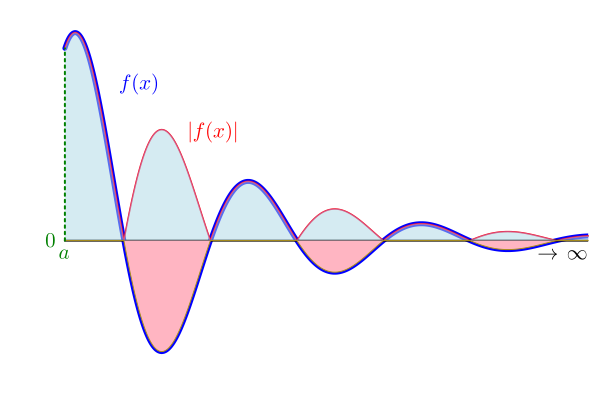
\includegraphics[width=0.6\columnwidth]{graphics/Chap08/ComparisonTest02.png}
\vspace*{-.4cm}
    \caption[]{\textbf{Absolute Integrability:} Suppose that $f:[a, \infty) \to \real$ is a piecewise continuous function so that its Riemann Integral exists and is finite for any bounded interval $[a, b]$. We observe that the area under $|f|$ is the sum of the area where $f\ge 0$ and THE NEGATIVE OF the area where $f\le 0$. Hence, if the area under $|f|$ is finite, then each of the positive (shaded blue) and negative (shaded pink) areas of $f$ must be finite, and therefore, the total area under $f$ is well-defined (aka, does not involve $\infty - \infty$) and finite.}
    \label{fig:AbsolutelyInegrable}
\end{figure}

\subsection{Absolute Integrability}

Consider a function $f:[a, \infty) \to \real$ that takes on both positive and negative values. As illustrated in Fig.~\ref{fig:AbsolutelyInegrable}, an easy way to make sense of its improper integral is to study the function's absolute value. Because the absolute value is non-negative, the comparison test can be applied. 

\bigskip

\begin{tcolorbox}[colback=mylightblue, title = {\bf Absolute Integrability}, breakable]
\begin{definition}
\label{def:AbsolutelyIntegrable}
A piecewise continuous function $f:[a, \infty) \to  \real$ is \textbf{absolutely integrable} if 
\begin{equation}
    \label{eq:AbsolutelyIntegrable}
    \int_a^\infty |f(x)| \, dx < \infty.
\end{equation}

\end{definition}

\end{tcolorbox}

\bigskip

\begin{propColor}{Usefulness of Absolute Integrability}{UsefulAbsoluteIntegrability}

Suppose that $f:[a, \infty) \to \real$ is piecewise continuous. Then the following hold:
\begin{enumerate}
\renewcommand{\labelenumi}{(\alph{enumi})}
\setlength{\itemsep}{.2cm}
    \item If $f$ is absolutely integrable, then $\int_a^\infty f(t) \, dt $ (without absolute value signs) exists and is finite.
    \item If $\displaystyle \lim_{t \to \infty} f(t)$ exists and is nonzero, then $f$ is not absolutely integrable.
    \item If $f$ is differentiable on $(a, \infty)$ and $f'$ (its derivative) is absolutely integrable, then $ \displaystyle \lim_{t \to \infty} f(t)$ exists and is finite. 
    \item If both $f$ and $f'$ (its derivative) are absolutely integrable on $(a, \infty)$, then $ \displaystyle \lim_{t \to \infty} f(t) = 0.$ 
\end{enumerate}

\bigskip
\textbf{Notes:} Each of these properties has its uses: (a) allows the comparison test to be used on functions that take on both positive and negative values; (b) provides a sufficient condition for a function NOT TO BE absolutely integrable; (c) provides a sufficient condition for a function to have a limit as $t$ goes to infinity; and (d) provides an extra condition for that limit to be zero.
    
\end{propColor}

\bigskip

\begin{figure}[htb]%
\centering
\hfill
\subfloat[]{%
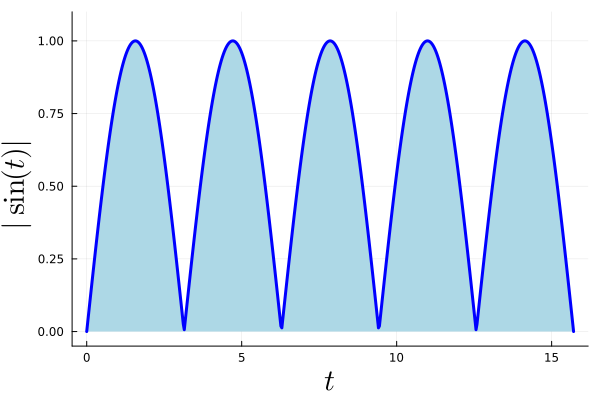
\includegraphics[width=0.4\columnwidth]{graphics/Chap08/plotShowsAbsSinNotAbsIntegrable.png}}%
\hfill%
\subfloat[]{%
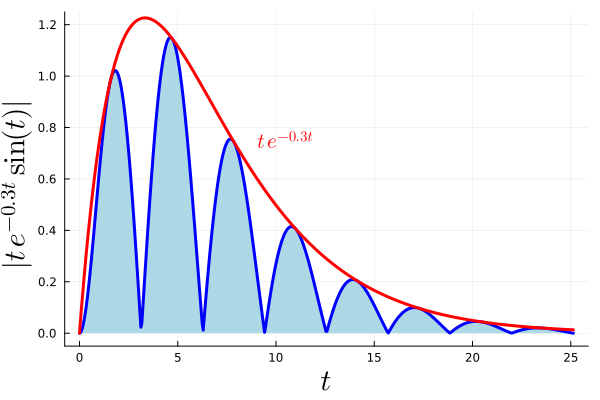
\includegraphics[width=0.4\columnwidth]{graphics/Chap08/plotShowWhenAbsTexpSinIsIntegrable.png}}%
\hspace*{1cm}
    \caption[]{\textbf{Common Functions and their Absolute Integrability:} (a) shows that $\sin(t)$ is not absolutely integrable over an unbounded interval, while (b) shows that a negative exponential damps out $t\, \sin(t)$ so that it becomes absolutely integrable; moreover, (b) also illustrates by the red line a decaying exponential eventually overtaking an exploding monomial. The same holds for higher powers of $t$.}
    \label{fig:CommonFunctionsAndTheirAbsoluteIntegrability}
\end{figure}
\bigskip
\begin{example} 
\label{ex:AbsoluteIntegrability}
Functions of the form $t^k\,e^{at}\, \sin(\omega t)$ and $t^k\,e^{at}\, \cos(\omega t)$ show up very often in engineering and STEM fields. Show that for all integers $k\ge 0$ and $\omega \in (0, \infty)$ that these functions are absolutely integrable on $[0, \infty)$ if, and only if, $a < 0$. 
\end{example}
\textbf{Solution:} The proofs for sine and cosine are identical, so we only give one of them. For $\sin(\omega t)$, it is important to exclude $\omega = 0$, while for $\cos(\omega t)$, it is not. The essence of the proofs can be deduced from Fig.~\ref{fig:CommonFunctionsAndTheirAbsoluteIntegrability}. If you understand the figure, you are good (the actual proof can then be an optional read); otherwise, read on.\\

\textbf{Part 1:} $a<0 \implies \int_0^\infty |t^k\,e^{at}\, \sin(\omega t) | \, dt < \infty.$ We break the proof into discrete steps to make it easier to follow.\\

\begin{itemize}
    \item $|t^k\,e^{at}\, \sin(\omega t)| \le t^k\,e^{at}\ $ for all $t\ge 0$ because $-1 \le \sin(\omega t) \le 1$ and $t^k\,e^{at}$ is non-negative. 
    \item Define $b:=\frac{|a|}{2}>0$ so that $a + b = \frac{a}{2} < 0$.
    \item Because $b>0$, and an exploding exponential dominates any monomial, there exists $0< T < \infty$ such that $t^k \le e^{bt}$ for all $t\ge T$.
    \item Putting these facts together, we arrive at  
    \begin{equation}
        \begin{aligned}
             \int_0^\infty |t^k\,e^{at}\, \sin(\omega t) | \, dt & \le  \int_0^\infty t^k\,e^{at} \, dt\\
             &\le  \int_0^T t^k\,e^{at} \, dt +  \int_T^\infty e^{bt}\,e^{at} \, dt \\
              &\le  \int_0^T t^k\,e^{at} \, dt +  \int_T^\infty e^{\frac{a}{2}t}  \, dt \\
             &\le \int_0^T t^k\,e^{at} \, dt +  \int_0^\infty e^{\frac{a}{2}t} \, dt,
        \end{aligned}
    \end{equation}
where the last line is true because integrating a positive function over a larger interval cannot decrease the value of the integral. 
\end{itemize}
The first integral is finite because we have a continuous function over a bounded interval. The second integral evaluates to $-\frac{2}{a}=\frac{2}{|a|}$, which is finite. Hence, the sum of the two integrals is finite, completing the proof.\\
 
\textbf{Part 2:} $a\ge 0 \implies \int_0^\infty |t^k\,e^{at}\, \sin(\omega t) | \, dt = \int_0^\infty t^k\,e^{at}\, |\sin(\omega t) | \, dt = \infty$. Again, we break the proof into discrete steps to make it easier to follow.\\

\begin{itemize}
    \item Let $T:=\frac{2 \pi}{\omega}>0$ be the period of $\sin(\omega T)$. 
    \item  $\displaystyle \int_0^\infty t^k\,e^{at}\, |\sin(\omega t) | \, dt := \lim_{N \to \infty} \int_0^{N\,T} t^k\,e^{at}\, |\sin(\omega t) | \, dt $.
    \item $\displaystyle  \int_0^{N\,T}t^k\,e^{at}\, |\sin(\omega t) | \, dt = \sum_{n=0}^{N-1} \int_{n\, T}^{(n+1)\, T} t^k\,e^{at}\, |\sin(\omega t) | \, dt$.
    \item Because $t^k\,e^{at}$ is non-decreasing\footnote{For $k>0$ or $a >0$, it is strictly increasing, but for $0=k=a$, it is constant.}, for all $n\ge 0$, $\displaystyle  \int_{n\, T}^{(n+1)\, T} t^k\,e^{at}\, |\sin(\omega t) | \, dt \ge \int_{0}^{T} t^k\,e^{at}\, |\sin(\omega t) | \, dt$.
    \item Hence, $\displaystyle  \sum_{n=0}^{N-1} \int_{n\, T}^{(n+1)\, T} t^k\,e^{at}\, |\sin(\omega t) | \, dt\ge \sum_{n=0}^{N-1} \int_{0}^{T} t^k\,e^{at}\, |\sin(\omega t) | \, dt = N \int_{0}^{T} t^k\,e^{at}\, |\sin(\omega t) | \, dt$.
\end{itemize}
Putting all of this together, 
\begin{equation}
    \begin{aligned}
         \int_0^\infty t^k\,e^{at}\, |\sin(\omega t) | \, dt & \ge \lim_{N \to \infty}  N \int_{0}^{T} t^k\,e^{at}\, |\sin(\omega t) | \, dt.
    \end{aligned}
\end{equation}
But, $\int_{0}^{T} t^k\,e^{at}\, |\sin(\omega t) | \, dt>0$ and hence, $\int_0^\infty t^k\,e^{at}\, |\sin(\omega t) | \, dt =\infty$.\\

Part 1 and Part 2 together prove the result.
\Qed.


\vspace*{1cm} 
\begin{figure}[ht]%
\centering
\subfloat[]{%
  \raisebox{0cm}[0pt][0pt]{%
    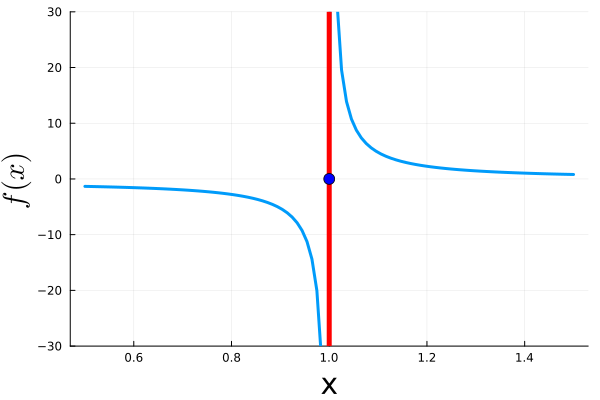
\includegraphics[width=0.45\columnwidth]{graphics/Chap08/plot_fx_near_plus1.png}%
  }%
}
\hfill%
\subfloat[]{%
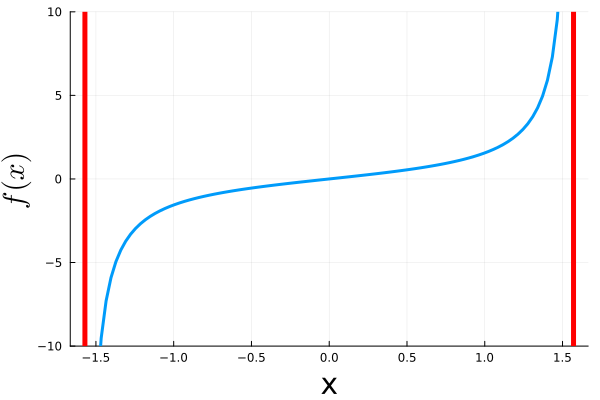
\includegraphics[ width=0.45\columnwidth]{graphics/Chap08/plot_tanx_near_origin.png} }
\hfill
    \caption[]{\textbf{Type-II Improper Integrals:} As shown in (a), the function $\frac{1}{x^2-1}$ has a vertical asymptote at $x=1$. Can we make sense of the integral $\int_0^1 \frac{1}{x^2-1} \, dx$ or  $\int_{0}^2 \frac{1}{x^2-1} \, dx$? Similarly, as shown in (b), the function $\tan(x)$ has vertical asymptotes at $x=\pm \frac{\pi}{2}$. Can we make sense of the integral $\int_0^{\frac{\pi}{2}} \tan(x) \, dx$? }
    \label{fig:TypeIIimproperIntegralVerticalAsymptotes}
\end{figure}


\section{Type-II Improper Integrals: Vertical Asymptotes}

If a function has a finite vertical asymptote, then it is diverging to $\pm \infty$ at some finite point $x_0\in \real$, as shown in Fig.~\ref{fig:TypeIIimproperIntegralVerticalAsymptotes}. As you can imagine, the unbounded nature of a function near a finite point demands extra attention when evaluating its integral, akin to situations where the limits of integration are unbounded. This Section is dedicated to exploring such integrals. \\

Before getting into the nitty-gritty, let's work through a few basic examples.\\

\bigskip
\textbf{Consider} $f:(0, 2) \to \real$ by $f(x) = \frac{1}{x^3}$. The function is continuous on the set $(0, 2)$, and for all $0<a <2$,  $\int_{a}^2 \frac{1}{x^3} \, dx$ exists and is finite. Indeed,
 $$\int_{a}^2 \frac{1}{x^3} \, dx = \int_{a}^2 x^{-3} \, dx = \frac{1}{-2} x^{-2} ~\bigg|_{a}^2 = \frac{1}{2x^2} ~\bigg|_{2}^a = \frac{1}{2a^2} -  \frac{1}{8}.$$
We next take the limit as $a$ approaches zero from the right, 
$$\int_{0}^2 \frac{1}{x^3} \, dx :=\lim_{a \to 0^+} \int_{a}^2 \frac{1}{x^3} \, dx = \lim_{a \to 0^+} \left( \frac{1}{2a^2} -  \frac{1}{8} \right) = \infty,$$
and hence, the integral is \textbf{divergent}. 

\bigskip
\textbf{Consider} $f:(0, 2) \to \real$ by $f(x) = \frac{1}{\sqrt{x}}$. The function is continuous on the set $(0, 2)$, and for all $0<a <2$,  $\int_{a}^2 \frac{1}{\sqrt{x}} \, dx$ exists and is finite. Indeed,
 $$\int_{a}^2 \frac{1}{\sqrt{x}} \, dx = \int_{a}^2 x^{-\frac{1}{2}} \, dx = \frac{1}{\frac{1}{2}} x^{\frac{1}{2}} ~\bigg|_{a}^2 = 2 \left(\sqrt{2}  - \sqrt{a} \right).$$
We next take the limit as $a$ approaches zero from the right, 
$$\int_{0}^2 \frac{1}{\sqrt{x}} \, dx :=\lim_{a \to 0^+} \int_{a}^2  \frac{1}{\sqrt{x}} \, dx = \lim_{a \to 0^+} 2 \left(\sqrt{2}  - \sqrt{a} \right) =  2 \cdot \sqrt{2},$$
and hence, the integral is \textbf{convergent}.

\bigskip
\textbf{Consider}  $f:[0, 1) \to \real$ by $f(x) = \frac{x}{ \sqrt[4]{1-x^2} }$, which has a vertical asymptote at $x_0 = 1$. The function is continuous on the set $(0, 1)$, and for all $0<b <1$,  $\int_{0}^b\frac{x}{\sqrt[4]{1-x^2}} \, dx$ exists and is finite. Indeed, we do the change of variable $u = 1-x^2 \implies du = -2x$, and compute
 $$\int_{x=0}^{x=b} \frac{x}{ \sqrt[4]{1-x^2} } \, dx = \int_{u=1}^{ u=1-b^2 } - \frac{1}{2} \frac{1}{ \sqrt[4]{u} } \, du=    \frac{1}{2} \int_{ u=1-b^2 }^{u=1} u^{ -\frac{1}{4} } \, du = 
\frac{1}{2} \frac{1}{ \frac{3}{4} } u^{ \frac{3}{4} } ~\bigg|_{u=1-b^2}^{u=1} = \frac{2}{3} \left(1 -  \left(1-b^2\right)^{ \frac{3}{4} } \right).$$
We next take the limit as $b$ approaches one from the left, 
$$\int_{0}^1  \frac{x}{ \sqrt[4]{1-x^2} }\, dx :=\lim_{b \to 1^-} \int_{0}^b  \frac{x}{ \sqrt[4]{1-x^2} }\, dx  = \lim_{b \to 1^-} \frac{2}{3} \left(1 -  \left(1-b^2\right)^{ \frac{3}{4} } \right) =  \frac{2}{3}.$$
and hence, the integral is \textbf{convergent}.

From the above, we see that the process is essentially identical to what we did for improper integrals of Type I: we set up the integral for a domain where the integrand is well-behaved (continuous and bounded), and then use a single-sided limit to approach the ``problematic point'' from the left or the right; for Type-I Integrals, the ``problematic point'' was $\pm \infty$, while for Type-II Integrals, it is $x_0{^+}$ or $x_0^-$, the right and left sides of a vertical asymptote. We'll do one more example to illustrate what happens when a vertical asymptote is strictly between the lower and upper bounds of integration, instead of being one of the endpoints of integration. 

\bigskip
\textbf{Consider}\footnote{Often, the person posing the problem will not be so careful as to define the function at the vertical asymptote, but they should be that careful.}  $f:[0, 2] \to \real$ by 
$$f(x) = \begin{cases} 
0 & x=1 \\
\frac{x}{ \sqrt[4]{|1-x^2|} } & \text{otherwise}
\end{cases},$$ where an absolute value was added to define the square root for $x>1$. The function is well behaved at each of the endpoints (does not blow up), so does the integral, $ \int_0^2 f(x) \, dx$, make sense? Especially when, as is often the case, it is written as 
$$ \int_0^2 \frac{x}{ \sqrt[4]{|1-x^2|} }  \, dx ?$$\\

The answer is: to make sense of it, we need to break the integral into two pieces, 
$$ \underbrace{\int_0^{1^-} \frac{x}{ \sqrt[4]{|1-x^2|} }  \, dx}_{\text{left of the asymptote}} + \underbrace{\int_{1^+}^2 \frac{x}{ \sqrt[4]{|1-x^2|} }  \, dx}_{\text{right of the asymptote}},$$
and then analyze each piece separately, just as we did with an integral having unbounded lower and upper limits. Then, as long as we can avoid the dreaded ``$\infty - \infty$'', we can sum the two answers and arrive at a value for the overall integral. If you think of $+\infty$ as approaching infinity from the left and $-\infty$ as approaching infinity from the right, then dealing with a Type-I Improper Integral with doubly infinite limits and a Type-II Improper Integral with an asymptote between the limits of integration, are really one and the same.

\begin{factColor}{Universal Approach for all Improper Integrals}{UniversalImproperIntegral}
To address an improper integral, the universal approach involves initially setting up a definite integral,
$$ \int_a^b f(x) \, dx, $$
where \( f: [a, b] \to \mathbb{R} \) is piecewise continuous and bounded. Subsequently,  evaluate the limit as \( a \) or \( b \) approaches either \( \pm \infty \) or converges to the left or right of a vertical asymptote. This process is done one limit at a time if both bounds of integration involve limits or if the original integral involves a vertical asymptote occurring at $a < x_0 < b$ (strictly between the limits).\\

\textcolor{blue}{\bf If you keep this process in mind, then there is no need to worry about Type-I vs Type-II Improper Integrals. In each case, taking a limit is your ``\href{https://en.wikipedia.org/wiki/Get_Out_of_Jail_Free_card}{get out of jail free card}''}. 
\end{factColor}


\bigskip
\begin{example} Evaluate the following integrals.
    \begin{enumerate}
\renewcommand{\labelenumi}{(\alph{enumi})}
\setlength{\itemsep}{.2cm}

 \item $\int_0 ^1 \frac{1}{x} \, dx$.
 
    \item $\int_0 ^1 \frac{1}{\sqrt{x}} \, dx$.

    \item $\int_0 ^2 \frac{1}{\sqrt[4]{|x-1|}}\, dx$.

    \item $\int_0 ^\frac{\pi}{2} \tan(x) \, dx$.

    \item $\int_{-1} ^1 \frac{x}{\sqrt{1 - x^2}} \, dx$.

\end{enumerate}
\end{example}
\textbf{Solutions:}

    \begin{enumerate}
\renewcommand{\labelenumi}{(\alph{enumi})}
\setlength{\itemsep}{.2cm}

 \item \Ans \quad $\int_0 ^1 \frac{1}{x} \, dx = \infty$.\\

 There is a vertical asymptote at $x_0=0$. Hence, $\int_0 ^1 \frac{1}{x} \, dx := \displaystyle \lim_{a \to 0^+} \int_a ^1 \frac{1}{x} \, dx = \lim_{a \to 0^+} \ln(x)~\bigg|_a^1 = \lim_{a \to 0^+} \left(\ln(1) -\ln(a) \right)= \infty$.
 
    \item \Ans \quad $\int_0 ^1 \frac{1}{\sqrt{x}} \, dx = 1$.\\

     There is a vertical asymptote at $x_0=0$. Hence, $\int_0 ^1 \frac{1}{\sqrt{x}} \, dx := \displaystyle \lim_{a \to 0^+} \int_a^1 x^{-\frac{1}{2}} \, dx = \lim_{a \to 0^+} \frac{1}{2} \sqrt{x}~\bigg|_a^1 = \lim_{a \to 0^+} \left(1 -\sqrt{a} \right)= 1$.

    \item \Ans \quad $\int_0 ^2 \frac{1}{\sqrt[4]{|x-1|}}\, dx =\frac{8}{3}$.\\

       There is a vertical asymptote at $x_0=1$. Hence, $\int_0 ^2 \frac{1}{\sqrt[4]{|x-1|}} \, dx := \int_0 ^{1^-} \frac{1}{\sqrt[4]{|x-1|}} \, dx +  \int_{1^+}^2 \frac{1}{\sqrt[4]{|x-1|}} \, dx$. Taking them one at a time gives
    \begin{align*}
        \int_0 ^{1^-} \frac{1}{\sqrt[4]{|x-1|}} \, dx &=  \lim_{b \to 1^-} \int_0^b \frac{1}{\sqrt[4]{|x-1|}} \, dx \\[1em]
        &=  \lim_{b \to 1^-} \int_0^b \frac{1}{\sqrt[4]{1-x}} \, dx ~~(\text{because }x-1\le 0 )\\[1em]
        &= \lim_{b \to 1^-} \int_0^b (1-x)^{-\frac{1}{4}} \, dx ~~(\text{prepare to apply generalized power rule})\\[1em]
         &= \lim_{b \to 1^-} \frac{1}{\frac{3}{4}}\cdot (-1)\cdot (1-x)^{\frac{3}{4}}~\bigg|_0^b ~~(\text{-1 is from the chain rule})\\[1em]
         & = \lim_{b \to 1^-} -\frac{4}{3} \left( (1-b)^{ \frac{3}{4} } - 1 \right)\\[1em]
         &= -\frac{4}{3} \left( (1-1)^{ \frac{3}{4} } - 1 \right)\\[1em]
         &= \frac{4}{3}
    \end{align*}
    and, next, 
        \begin{align*}
        \int_{1^+}^2 \frac{1}{\sqrt[4]{|x-1|}} \, dx &=  \lim_{a \to 1^+} \int_a^2 \frac{1}{\sqrt[4]{|x-1|}} \, dx \\[1em]
        &=  \lim_{a \to 1^+}  \int_a^2  \frac{1}{\sqrt[4]{x-1}} \, dx ~~(\text{because }x-1\ge 0 )\\[1em]
        &= \lim_{a \to 1^+} \int_a^2  (1-x)^{-\frac{1}{4}} \, dx ~~(\text{prepare to apply generalized power rule})\\[1em]
         &= \lim_{a \to 1^+}  \frac{1}{\frac{3}{4}}\cdot (1-x)^{\frac{3}{4}}~\bigg|_a^2 \\[1em]
         & = \lim_{a \to 1^+}  \frac{4}{3} \left( (2-1)^{ \frac{3}{4} } -  (a-1)^{ \frac{3}{4} }  \right)\\[1em]
         & = \frac{4}{3} \left( (2-1)^{ \frac{3}{4} } -  (1-1)^{ \frac{3}{4} }  \right)\\[1em]
         &= \frac{4}{3}.
    \end{align*}    
       Hence, $\int_0 ^2 \frac{1}{\sqrt[4]{|x-1|}}\, dx = \frac{4}{3}  + \frac{4}{3} = \frac{8}{3}$.\\

   \textbf{Note:} In the first integral, you can do a u-substitution, via, $u = 1-x \implies du = -dx$
  \begin{align*}
      \int_{x=0}^{x=b} (1-x)^{-\frac{1}{4}} \, dx &= \int_{u=1}^{u=1-b} u^{-\frac{1}{4}} \, (-1)\, du \\[1em]
      &= \int_{u=1-b}^{u=1}  u^{-\frac{1}{4}} \, du ~~(\text{swap bounds of integration to remove minus sign}) \\[1em]
      &= \frac{4}{3} u^{\frac{3}{4}} ~\bigg|_{1-b}^{1}.
  \end{align*} 
      

    \item \Ans \quad  $\int_0 ^\frac{\pi}{2} \tan(x) \, dx =\infty$. \\

    There is a vertical asymptote at $x_0 = \frac{\pi}{2}$. Before dealing with that, let's obtain an antiderivative for $\tan(x) = \frac{\sin(x)}{\cos(x)}$ via the u-substitution, $u = \cos(x) \implies du = -\sin(x) \, dx$. Hence,
    $$ \int \frac{\sin(x)}{\cos(x)}\, dx = \int -\frac{1}{u} du = -\ln(u) +C = -\ln(\cos(x)) + C.$$
    Knowing the antiderivative, we compute
    \begin{align*}
        \int_{0}^{ \frac{\pi}{2} } \tan(x) \, dx &= \lim_{ b \to \frac{\pi}{2}^- }  \int_{0}^{b} \tan(x) \, dx  \\[1em] 
        &= \lim_{ b \to \frac{\pi}{2}^- }  -\ln(\cos(x)) ~\bigg|_{0}^{b} \\[1em]
         &= \lim_{b \to \frac{\pi}{2}^-}  \ln(\cos(x)) ~\bigg|_{b}^0 ~~(\text{swap bounds of integration to remove minus sign}) \\[1em]
         &=  \lim_{b \to \frac{\pi}{2}^-} \left( \ln(\cos(0))  - \ln(\cos(b))  \right) \\[1em]
         &= 0 - (-\infty)\\
         &=\infty.         
    \end{align*}

    \textbf{Note:} If you were to compute $\displaystyle \int_{-\frac{\pi}{2}}^{ \frac{\pi}{2} } \tan(x) \, dx $, you would have two vertical asymptotes, one at $ -\frac{\pi}{2}$ and one at  $ \frac{\pi}{2}$, and you would arrive at the integral being undefined due to $-\infty + \infty$. If you have trouble seeing this, do a quick plot of $\tan: (-\frac{\pi}{2}, \frac{\pi}{2}) \to \real$.

    \item \Ans \quad $\int_{-1} ^1 \frac{x}{\sqrt{1 - x^2}} \, dx = 0$.\\

    There are vertical asymptotes at $\pm 1$. Before dealing with that, let's find an antiderivative for $\frac{x}{\sqrt{1 - x^2}}$ via the u-substitution $u = 1-x^2 \implies du = -2x \, dx$. Hence, 
    \begin{align*}
        \int \frac{x}{\sqrt{1 - x^2}} \, dx & = \int-\frac{1}{2} \frac{1}{\sqrt{1 - x^2}} \,(-2x)\, dx \\[1em]
        &=\int -\frac{1}{2}\frac{1}{\sqrt{u}} \, du \\[1em]
        &= \int -\frac{1}{2} u^{-\frac{1}{2}} \, du  \\[1em]
        &=  -\frac{1}{2} \cdot \frac{1}{\frac{1}{2}}u^{\frac{1}{2}} + C \\[1em]
        & = - \sqrt{u} + C \\
        & = - \sqrt{1-x^2} + C \\
    \end{align*}

    Now that we have an antiderivative, $\int_{-1} ^1 \frac{x}{\sqrt{1 - x^2}} \, dx = \displaystyle \lim_{a \to -1^+} \int_a^0  \frac{x}{\sqrt{1 - x^2}} \, dx +  \lim_{b \to 1^-} \int_0^b  \frac{x}{\sqrt{1 - x^2}} \, dx$. Taking the integrals one at a time, we have, for the first integral,
       \begin{align*}
        \lim_{a \to -1^+} \int_a^0  \frac{x}{\sqrt{1 - x^2}} \, dx & = \lim_{a \to -1^+} - \sqrt{1 - x^2}~\bigg|_a^{0} \\[1em]
        &= \lim_{a \to -1^+}  \sqrt{1 - x^2}~\bigg|_{0}^a ~~(\text{swap bounds of integration to remove minus sign}) \\[1em]
        &=  \lim_{a \to -1^+} \left( \sqrt{1 - a^2} - \sqrt{1 - 0}\right) \\[1em]
        &= \frac{1}{4}  \left( \sqrt{1 - 1} - \sqrt{1 }\right) \\[1em]
        & = -1.
    \end{align*}

    Evaluating the second integral,
     \begin{align*}
        \lim_{b \to 1^-} \int_0^b  \frac{x}{\sqrt{1 - x^2}} \, dx & =\lim_{b \to 1^-} - \sqrt{1 - x^2}~\bigg|_0^{b} \\[1em]
        &= \lim_{b \to 1^-}  \sqrt{1 - x^2}~\bigg|_b^0 ~~(\text{swap bounds of integration to remove minus sign}) \\[1em]
        &=  \lim_{b \to 1^-}   \left( \sqrt{1 - 0} - \sqrt{1 - b^2}\right) \\[1em]
        &= \lim_{b \to 1^-} \left( 1 - \sqrt{1 -1}\right) \\[1em]
        & = 1.
    \end{align*}

    Hence, $\int_{-1} ^1 \frac{x}{\sqrt{1 - x^2}} \, dx = \displaystyle \lim_{a \to -1^+} \int_a^0  \frac{x}{\sqrt{1 - x^2}} \, dx +  \lim_{b \to 1^-} \int_0^b  \frac{x}{\sqrt{1 - x^2}} \, dx = -1 + 1 =0$.

\end{enumerate}

\Qed

\bigskip

\begin{example} Use, or attempt to use, \texttt{quadgk} to evaluate the following integrals. The primary goal is to determine whether it detects that there is a ``problem'' due to its integrand blowing up over the domain of integration or not. A secondary goal would be to estimate the value of the integral using \texttt{quadgk}. 
    \begin{enumerate}
\renewcommand{\labelenumi}{(\alph{enumi})}
\setlength{\itemsep}{.2cm}

\item $\int_0 ^1 \frac{1}{x} \, dx$.
 

\item $\int_{-2}^2 \frac{x}{\sqrt{1 - x^2}} \, dx$, has two vertical asymptotes within the domain of integration.

\end{enumerate}
\end{example}
\textbf{Solutions:}

a) We apply numerical techniques to $\int_0 ^1 \frac{1}{x} \, dx.$

\begin{lstlisting}[language=Julia,style=mystyle]
using QuadGK
fa(x) = 1/x
sol,  = quadgk(fa, 0, 1)
\end{lstlisting}
\textbf{Output} 
\begin{verbatim}
DomainError with 3.5601181736115222e-307:
integrand produced Inf in the interval (0.0, 7.120236347223045e-307)
\end{verbatim}

That is reassuring: \texttt{quadgk} detected there is an issue. So, we ask next, can we use \texttt{quadgk} to determine if the integral is convergent or divergent? 

\begin{lstlisting}[language=Julia,style=mystyle]
using QuadGK
k=collect(1:2:10)
limitRange = 10.0.^(-k)
for a in limitRange
    sol,  = quadgk(fa, a, 1)
    display([a sol])
end
\end{lstlisting}
\textbf{Output} 
\begin{verbatim}
1×2 Matrix{Float64}:
 0.1  2.30259
1×2 Matrix{Float64}:
 0.001  6.90776
1×2 Matrix{Float64}:
 1.0e-5  11.5129
1×2 Matrix{Float64}:
 1.0e-7  16.1181
1×2 Matrix{Float64}:
 1.0e-9  20.7233
\end{verbatim}
Once again, this is reassuring: as $a\to 0^+$, the integral is not converging. It would take a lot to show that it is really divergent, but we are getting a hint of it, at least.\\

b) We apply numerical techniques to $\int_{-2}^2 \frac{x}{\sqrt{1 - x^2}} \, dx$, which has vertical asymptotes at $\pm 1$.
\begin{lstlisting}[language=Julia,style=mystyle]
using QuadGK
fe(x) = x/sqrt(abs(1 - x^2))
# There are two vertical asymptotes within the domain of integration 
sol,  = quadgk(fe, -2, 2) 
\end{lstlisting}
\textbf{Output} 
\begin{verbatim}
DomainError with -1.0:
integrand produced NaN in the interval (-2.0, 0.0)
\end{verbatim}
Sweet! It caught the first vertical asymptote at $x_0 = -1$, even though it was not on the boundary. We push our luck and continue.\\

\begin{lstlisting}[language=Julia,style=mystyle]
using QuadGK
fe(x) = x/sqrt(abs(1 - x^2))
# There remains one vertical asymptote within the domain of integration 
sol,  = quadgk(fe, -0.99, 2) # -0.99 approx = -1^+ = -1 + a tiny bit
\end{lstlisting}
\textbf{Output} 
\begin{verbatim}
(1.8731177232031915, 2.1226263027166235e-8)
\end{verbatim}
\textcolor{red}{\bf It does not complain about the vertical asymptote at $+1$.} \\
\begin{lstlisting}[language=Julia,style=mystyle]
using QuadGK
fe(x) = x/sqrt(abs(1 - x^2))
# There remains one vertical asymptote within the domain of integration 
sol,  = quadgk(fe, -1.0+1e-4, 2) # -0.9999 approx = -1^+ = -1 + a tiny bit
\end{lstlisting}
\textbf{Output} 
\begin{verbatim}
(1.746192377358709, 2.5638760207248433e-8)
\end{verbatim}
\textcolor{blue}{\bf As we will see later, that is a very good approximation of the integral. QuadGK has integrated through the singularity. You can play with the code and try \texttt{sol,  = quadgk(fe, -1.0+1e-6, 2)}  to see what happens.}\\


\textbf{We know where the vertical asymptotes are. Let's see how \texttt{quadgk} does if we use that information.}\\

$\int_{-2}^{-1^-} \frac{x}{\sqrt{1 - x^2}} \, dx$ \\

\begin{lstlisting}[language=Julia,style=mystyle]
# Integrate from -2 to -1
using QuadGK
k=collect(1:3:15)
epsilonRange = 10.0.^(-k)
b=-1
for epsilon in epsilonRange
    sol,  = quadgk(fe, -2, b-epsilon)
    display([b-epsilon sol])
end
\end{lstlisting}
\textbf{Output} 
\begin{verbatim}
1×2 Matrix{Float64}:
 -1.1  -1.27379
1×2 Matrix{Float64}:
 -1.0001  -1.71791
1×2 Matrix{Float64}:
 -1.0  -1.7316
1×2 Matrix{Float64}:
 -1.0  -1.73204
1×2 Matrix{Float64}:
 -1.0  -1.73205
\end{verbatim}
Awesome! We get that $\int_{-2}^{1^-}  \frac{x}{\sqrt{1 - x^2}} \, dx \approx  -1.73205$. Next, we are going to cheat a bit and go for 
$ \int_{-1^+}^{1^-}  \frac{x}{\sqrt{1 - x^2}} \, dx$. We should break it into two integrals, over $[-1^+, 0]$ and $[0, 1^-]$, but what the heck, let's roll the dice, something a real engineer would never do, right?
\begin{lstlisting}[language=Julia,style=mystyle]
# Integrate from -1 to +1
using QuadGK
k=collect(1:3:15)
epsilonRange = 10.0.^(-k)
a = -1
b = 1
for  epsilon in epsilonRange
    sol,  = quadgk(fe, a + epsilon, b - epsilon)
    display([a + epsilon b - epsilon sol])
end
\end{lstlisting}
\textbf{Output} 
\begin{verbatim}
1×3 Matrix{Float64}:
 -0.9  0.9  4.66156e-17
1×3 Matrix{Float64}:
 -0.9999  0.9999  1.93258e-16
1×3 Matrix{Float64}:
 -1.0  1.0  1.19294e-15
1×3 Matrix{Float64}:
 -1.0  1.0  6.37856e-16
1×3 Matrix{Float64}:
 -1.0  1.0  -1.35308e-16
\end{verbatim}
Sweet, we get zero. Finally, we go for $\int_{1^+}^{2}  \frac{x}{\sqrt{1 - x^2}} \, dx$


\begin{lstlisting}[language=Julia,style=mystyle]
# Integrate from +1 to +2
using QuadGK
k=collect(1:3:15)
epsilonRange = 10.0.^(-k)
a = 1
b = 2
for  epsilon in epsilonRange
    sol,  = quadgk(fe, a + epsilon, b - epsilon)
    display([a + epsilon b - epsilon sol])
end
\end{lstlisting}
\textbf{Output} 
\begin{verbatim}
1×3 Matrix{Float64}:
 1.1  1.9  1.15729
1×3 Matrix{Float64}:
 1.0001  1.9999  1.71779
1×3 Matrix{Float64}:
 1.0  2.0  1.7316
1×3 Matrix{Float64}:
 1.0  2.0  1.73204
1×3 Matrix{Float64}:
 1.0  2.0  1.73205
\end{verbatim}
And we obtain $\int_{1^+}^{2}  \frac{x}{\sqrt{1 - x^2}} \, dx \approx 1.73205$. When we add up all the pieces, we obtain zero. 

\Qed

\textcolor{blue}{\bf Bottom line:} QuadGK is a valid option for evaluating improper integrals, though additional care is required. 


\bigskip
\textbf{Recommended Videos for Additional Practice}
\begin{itemize}
    \item \href{https://youtu.be/w46sjRIkV7Y}{8 Examples of Type II Improper Integrals, Calculus 2)} by \bprp.
    \item \href{https://youtu.be/C24iWgk28EU}{Type II Improper Integrals - Discontinuous Integrands - Convergence and Divergence} by K.O. Math has very nice graphics to help with intuition.
    \item \href{https://youtu.be/sjlZ_KX3cqM}{Type I vs Type II Improper Integrals (10 examples)} by \bprp.
    \item \href{https://youtu.be/oq46Nl8W1H0}{Improper Integrals (6 of 16) Type 2 Example} by Prof. Michel van Biezen.
\end{itemize}

\section{Improper Integrals through the Lens of Probability}

Improper integrals are common in probability theory, the ``science of randomness''. 

\bigskip

\begin{funColor}{Understanding Randomness through Exam Scores}{WhatIsRandomness}
Imagine you're about to take an important exam. You might think that your score will depend solely on how well you've studied. However, even if you're fully prepared, there are countless unforeseen factors that could influence your performance. These factors introduce an element of \textbf{randomness} into what your final score might be, where \textbf{randomness} refers to the outcome of events that are not certain and the complex ways in which these uncertain events influence outcomes. It's a concept found everywhere around us, from the roll of dice to the weather each day.\\

\textbf{Exam Score Factors:} Consider your score on an exam as a random variable. This doesn't mean your score is entirely left to chance; rather, it's affected by a combination of predictable elements (like how much you studied) and unpredictable ones (randomness), such as the factors listed below:

\begin{itemize}
  \item \textbf{Did You Sleep Well?} A good night's sleep is crucial for memory and concentration. Poor sleep could unexpectedly lower your performance.
  
  \item \textbf{Transportation Troubles}: Being late because the bus was delayed can cause panic and rush, impacting your focus and, consequently, your score.
  
  \item \textbf{Unexpected News}: Receiving distressing news from a friend right before the exam can unsettle you, or on the flip side, hearing good news (like winning the lottery) might overly excite you, both affecting your concentration.
  
  \item \textbf{Personal Well-being}: Sudden headaches, feeling unwell, or even the room being too cold or too hot can distract you during the exam.

   \item \textbf{Antsy People Near You}: A nearby student who twiddles their pencil or keeps moving around in their chair can cause a loss of concentration. 

   \item \textbf{Order the Questions are Placed on the Exam}: Nailing the first question can give you a sense of calm for proceeding to the next questions, while flailing away on the first question can undermine your confidence.

   \item \textbf{Adequate Time to Study:} Maybe you have a job and had to work overtime, or another course scheduled its exam on the same day with very little notice. 
\end{itemize}


You would agree that most of the factors listed above are not in your direct control and that you cannot predict ahead of time with any degree of certainty whether or not they will occur for you on any given exam. That is what randomness is all about. It's a concept that stretches far beyond the simple outcome of flipping a coin or rolling dice. Randomness infiltrates every aspect of our lives, influencing events in ways that are often subtle, sometimes profound, and always unavoidable.\\

The subjects of \textbf{Probability} and \textbf{Statistics} are the mathematical siblings born out of the need to understand and quantify this randomness. Through these disciplines, humanity has developed a toolkit not just for gauging the likelihood of events but also for making sense of the random variability that surrounds us. You have likely heard the terms $\textbf{mean}$, $\textbf{variance}$, and $\textbf{standard deviation}$, which are critical in this endeavor. Let's delve a bit deeper into how these quantities help us grapple with randomness:

\begin{itemize}
    \item The $\textbf{mean}$, often referred to as the average, gives us a central value for a set of data. When considering exam scores across many students, the mean score provides a quick snapshot of the overall performance level.
    \item $\textbf{Variance}$ measures how spread out a set of data is. If we're looking at the variance in exam scores, we're essentially asking, ``How much do students' scores differ from each other and from the mean?'' High variance means a wide dispersion of scores, indicating that factors of randomness may have had varied impacts on the students.
    \item The $\textbf{standard deviation}$, the square root of the variance, offers a digestible measure of this spread in the same units as the data itself. It tells us, on average, how far each student's exam score deviates from the mean score. Understanding standard deviation allows students to appreciate the diversity of outcomes produced by both controllable factors (like study habits) and uncontrollable factors (like those random events we discussed).
\end{itemize}

Through Probability and Statistics, engineers learn to model, analyze, and interpret the effects of randomness. We use these mathematical methods to study random events, enabling us to predict probabilities, assess risks, and make informed decisions—even in the face of uncertainty. So, while we might not be able to control or predict every factor that affects our lives, these disciplines give us a powerful way to understand and manage the complexity of randomness.
  
\end{funColor}

\subsection{What is a Probability Density?}

In formal courses on Probability and Statistics, you'll explore different ways to model (aka, mathematically represent) random quantities, including probability measures, distributions, and densities. This section highlights \textbf{probability densities}--functions \(f: \mathbb{R} \to [0, \infty)\) that are non-negative, sum up (integrate) to one, and where the integral \(\int_a^b f(x) \, dx\) signifies the probability of a random quantity falling within the range $[a, b]$, such as your exam score being between 86\% and 93\%. Some probability densities are defined on bounded sets, and others on unbounded sets. Those defined on unbounded sets require improper integrals.



\subsection{The Role of Improper Integrals}

Consider a web server where events correspond to users requesting information. The time between one user request and the next is a random variable. The time between these events is often modeled using the \href{https://en.wikipedia.org/wiki/Exponential_distribution}{exponential distribution}, a choice motivated by its so-called ``memoryless property'': the probability of the next event occurring does not depend on how much time has elapsed since the previous event occurred.

\bigskip

\begin{example}
The probability density function (PDF) for the exponential distribution is given by
\[ f(x) = \lambda e^{-\lambda x}, \]
where \(\lambda > 0\) is the rate parameter, and \(x \ge 0\) represents the time between events in clock cycles. Given the high clock frequencies of modern processors, the time \(x\) can stretch towards infinity, making this an example of an improper integral. For the exponential distribution, do the following:
\begin{enumerate}
\renewcommand{\labelenumi}{(\alph{enumi})}
\setlength{\itemsep}{.2cm}
    \item Show the PDF integrates to one.
    \item Compute the mean value.
    \item Compute the variance.
\end{enumerate}
\end{example}

\textbf{Solution:}

\begin{enumerate}
\renewcommand{\labelenumi}{(\alph{enumi})}
\setlength{\itemsep}{.2cm}
    \item We need to show $\displaystyle \int_0^\infty \lambda e^{-\lambda x} \, dx = 1$. 
Let's compute this integral, considering it as an improper integral due to the infinite upper bound.

\[
\begin{aligned}
\int_0^\infty \lambda e^{-\lambda x} \, dx &= \lim_{t \to \infty} \int_0^t \lambda e^{-\lambda x} \, dx \\
&= \lim_{t \to \infty} \left[-e^{-\lambda x}\right]_0^t \\
&= \lim_{t \to \infty} \left(-e^{-\lambda t} + e^{-\lambda \cdot 0}\right) \\
&= \lim_{t \to \infty} \left(-e^{-\lambda t} + 1\right) \\
&= 1.
\end{aligned}
\]
    \item In a course on Probability and Statistics, you will learn that the mean value, often denoted by $\mu$, satisfies
\[ \mu = \int_0^\infty x f(x) \, dx. \]
Specializing this formula to the exponential distribution gives
\[ \mu = \int_0^\infty x \lambda e^{-\lambda x} \, dx. \]

To find the mean value $\mu$, we use integration by parts, where $u = x$ and $dv = \lambda e^{-\lambda x} dx$, giving $du = dx$ and $v = -e^{-\lambda x}$. Thus,
\[
\begin{aligned}
\mu &= \left. -xe^{-\lambda x} \right|_0^\infty + \int_0^\infty e^{-\lambda x} \, dx \\
&= \lim_{t \to \infty} \left( -te^{-\lambda t} \right) + \left[ -\frac{1}{\lambda}e^{-\lambda x} \right]_0^\infty \\
&= 0 + \left( 0 - \left(-\frac{1}{\lambda}\right) \right) \\
&= \frac{1}{\lambda}.
\end{aligned}
\]

    \item In a course on Probability and Statistics, you will learn that the variance, often denoted by $\sigma^2$, satisfies 
     \[ \sigma^2 = \int_0^\infty (x - \mu)^2 f(x) \, dx. \]
Specializing this formula to the exponential distribution gives    
    \[ \sigma^2 = \int_0^\infty (x - \mu)^2 \lambda e^{-\lambda x} \, dx. \]

To find the variance $\sigma^2$, we first substitute in $\mu = \frac{1}{\lambda}$ and then expand the quadratic, giving, 
\[ \sigma^2 = \int_0^\infty (x - \frac{1}{\lambda})^2  \lambda e^{-\lambda x}  \, dx = \int_0^\infty x^2 \lambda e^{-\lambda x} \, dx - 2\, \frac{1}{\lambda} \int_0^\infty x \lambda e^{-\lambda x} \, dx + \left(\frac{1}{\lambda} \right)^2 \int_0^\infty \lambda e^{-\lambda x} \, dx. \]
The second and third terms have been computed in part (b) and part (a) respectively. For the first term, using integration by parts twice (details left as an exercise), we find:
\[ \int_0^\infty x^2 \lambda e^{-\lambda x} \, dx = \frac{2}{\lambda^2}. \]
Thus,
\[ \sigma^2 = \frac{2}{\lambda^2} - 2\left(\frac{1}{\lambda}\right)\left(\frac{1}{\lambda}\right) + \left(\frac{1}{\lambda}\right)^2 = \frac{1}{\lambda^2}. \]
\end{enumerate}

\Qed
\bigskip

We focus next on the normal distribution, which is one of the most fundamental distributions in probability and statistics due to the \href{https://en.wikipedia.org/wiki/Central_limit_theorem}{Central Limit Theorem}. Unlike the exponential distribution example, the integration to show that the normal distribution density integrates to one is complex and typically beyond the scope of a first calculus course. Thus, we'll concentrate on verifying the mean.

\begin{example}
The probability density function (PDF) for the normal distribution is given by:
\[ f(x) = \frac{1}{\sigma\sqrt{2\pi}} e^{-\frac{1}{2}\left(\frac{x-\mu}{\sigma}\right)^2}, \]
where \(\mu\) is (supposed to represent) the mean, \(\sigma\) is (supposed to be) the standard deviation, and \(x \in \real\) represents the value of the random variable. Verify that the mean value really is given by $\mu$.
\end{example}

\textbf{Solution:} 

The integral to find the mean $\mu$ is
\[ \mu =\int_{-\infty}^{\infty} x \cdot \frac{1}{\sigma\sqrt{2\pi}} e^{-\frac{1}{2}\left(\frac{x-\mu}{\sigma}\right)^2} dx. \]
This is a doubly improper integral. We break it into two parts
\begin{align*}
    \int_{\mu}^{\infty} x \cdot \frac{1}{\sigma\sqrt{2\pi}} e^{-\frac{1}{2}\left(\frac{x-\mu}{\sigma}\right)^2} dx &:= \lim_{b \to \infty} \int_{\mu}^{b} x \cdot \frac{1}{\sigma\sqrt{2\pi}} e^{-\frac{1}{2}\left(\frac{x-\mu}{\sigma}\right)^2} dx, \\
     \int_{-\infty}^{\mu} x \cdot \frac{1}{\sigma\sqrt{2\pi}} e^{-\frac{1}{2}\left(\frac{x-\mu}{\sigma}\right)^2} dx &:= \lim_{a \to -\infty} \int_{a}^{\mu} x \cdot \frac{1}{\sigma\sqrt{2\pi}} e^{-\frac{1}{2}\left(\frac{x-\mu}{\sigma}\right)^2} dx.
\end{align*}
Focusing on the first integral, substitute $z = \frac{x-\mu}{\sigma}$, thus $dx = \sigma dz$, and $x = \mu + \sigma z$, yielding
\[ \lim_{b \to \infty} \int_{0}^{\frac{b-\mu}{\sigma}} (\mu + \sigma z) \frac{1}{\sqrt{2\pi}} e^{-\frac{1}{2}z^2} \sigma dz. \]

Splitting the integral gives
\[  \lim_{b \to \infty}\, \mu \, \int_{0}^{\frac{b-\mu}{\sigma}} \frac{1}{\sqrt{2\pi}} e^{-\frac{1}{2}z^2} \sigma dz + \lim_{b \to \infty}\, \sigma  \, \int_{0}^{\frac{b-\mu}{\sigma}} z\, \frac{1}{\sqrt{2\pi}} e^{-\frac{1}{2}z^2} \sigma dz. \]
To evaluate the first integral, you have to know that the integral of the Gaussian density is one, and half of the Gaussian density gives $\frac{1}{2}$. The second integral can be done by u-substiution and yields one. Hence, 
\[\lim_{b \to \infty} \int_{0}^{\frac{b-\mu}{\sigma}} (\mu + \sigma z) \frac{1}{\sqrt{2\pi}} e^{-\frac{1}{2}z^2} \sigma dz = \frac{\mu}{2} + \sigma. \]

The second integral is similar and yields, 
$$\lim_{a \to -\infty} \int_{a}^{\mu} x \cdot \frac{1}{\sigma\sqrt{2\pi}} e^{-\frac{1}{2}\left(\frac{x-\mu}{\sigma}\right)^2} dx = \frac{\mu}{2} - \sigma.$$
Adding them up, completes the verification.


\Qed

\bigskip 
\begin{example} While proving that the Gaussian density really does integrate to one is a bit advanced for a first Calculus course, showing that the integral exists and is bounded is much easier. So that you can focus on the essential elements, prove that $\int_0^\infty e^{-x^2} \, dx$ exists and is finite.    
\end{example}
\solution We use the Comparison Test. For $x\ge 1$, $e^{-x^2} \le x\, e^{-x^2}$. Hence, 
\begin{align*}
    \int_1^\infty e^{-x^2} \, dx & \le \int_1^\infty x \, e^{-x^2} \, dx \\[1em]
    &\le  \int_0^\infty x \, e^{-x^2} \, dx ~~(\text{because the integrand is non-negative}) \\[1em] 
    & \le  \frac{1}{2} \int_0^\infty e^{-u} \, du ~~(\text{u-substitution } u = x^2, du = 2x dx) \\[1em]
    &\le  \frac{1}{2}\, e^{-u} \Big|_{0}^{\infty} \\[1em]
    &\le  \frac{1}{2}.
\end{align*}

Because $e^{-x^2}$ is continuous, $\int_0^1 e^{-x^2} \, dx$ exists and is finite. Hence, by combining this with the previous bound, we obtain the desired result.\\

Alternatively, one can apply the Comparison Test like this: for $x\ge 1$, $e^{-x^2} \le e^{-x}$. We ask the learner to adapt the above proof to this new bound.
\Qed.

\bigskip

Functions of the form $c \, \frac{1}{x^k}$, $x \ge x_{\rm min}>0$ are called \textbf{power-law densities} or \textbf{Pareto} densities. They occur in Psychology to model forgetting, Climate Science to model energy dissipation in cyclones, in Computer Engineering to model the relationship between a CPU's cache size and the number of cache misses, and in Economics to model relationships varying from the distribution of artists by the average price of their artworks to income distribution in a market economy.

\bigskip

\begin{example} Assume a power-law density $f(x) = c \, \frac{1}{x^3}$, $x \in [1, \infty)$. Do the following:
\begin{enumerate}
\renewcommand{\labelenumi}{(\alph{enumi})}
\setlength{\itemsep}{.2cm}
    \item Find $c$ such that $f$ is a density.
    \item Compute the mean value.
    \item Compute the variance.
\end{enumerate}
\end{example}

\solution
\begin{enumerate}
\renewcommand{\labelenumi}{(\alph{enumi})}
\item To find $c$ such that $f$ is a density, we integrate $f(x)$ over its domain and set the integral equal to 1, namely
\[ 1 = \int_{1}^{\infty} c \, \frac{1}{x^3} \, dx = c \frac{x^{-2}}{-2} \Bigg|_{1}^{\infty}  = \frac{c}{2}.\]
Solving this, we find $c = 2$.

\item The mean value $\mu$ is computed as,
 \[ \mu = \int_{1}^{\infty} x f(x) \, dx = \int_{1}^{\infty} x \, \frac{2}{x^3} \, dx  = 2 \, \frac{ x^{-1} }{-1} \Bigg|_{1}^{\infty} = 2. \]

\item The variance $\sigma^2$ is theoretically obtained  via,
\[ \sigma^2 = \int_{1}^{\infty} (x - \mu)^2 f(x) \, dx.\]
However, the improper integral is divergent. In a course on Probability, one would say that the infinite variance is due to the power-law's ``heavy tail'' (meaning, the tail of the density does not drop off to zero rapidly enough to yield a finite integral). \\

To see qualitatively that the integral is divergent, note that $x^2$ times $\frac{1}{x^3}$ behaves like $\frac{1}{x}$, which is the line of demarcation for convergent and divergent integrals, as shown in the preliminaries to Chapter~\ref{sec:ComparisonTest}.  To show divergence analytically, note that
$$ (x - \mu)^2 f(x) = \left(x^2 - 2 \mu x + \mu^2  \right) \, \frac{2}{x^3},$$
and that
$$ \int_1^\infty x^2 \frac{2}{x^3} \, dx = \int_1^\infty \frac{2}{x} \, dx = 2 \ln(x) \Big|_1^\infty = \infty,$$
while $$  \int_1^\infty (- 2 \mu x ) \frac{2}{x^3} \, dx =  -4 \, \int_1^\infty x \, \frac{2}{x^3} \, dx = -8$$
and
$$ \int_1^\infty \mu^2 \,  \frac{2}{x^3} \, dx = 4 \, \int_1^\infty x \, \frac{2}{x^3} \, dx = 8.$$
We did the last two integrals just to assure you that we did not land in $\infty - \infty$, which would have landed us in the ``undefined'' category, instead of divergent. If that seems like splitting hairs to you, for most engineering applications, you're probably right!
\end{enumerate}
\Qed

In Michigan's IOE 265 \textit{Probability and Statistics for Engineers} or EECS 301 \textit{Probabilistic Methods in Engineering}, you will encounter integration challenges similar to the above.


\section{(Optional Read:) Proofs Associated with the Chapter}

\begin{tcolorbox}[title=\textcolor{black}{Proof of Prop.~\ref{thm:UsefulAbsoluteIntegrability} (Usefulness of Absolute Integrability}, sharp corners, colback=green!30, colframe=green!80!blue, breakable, fonttitle=\bfseries]
Suppose that $f:[a, \infty) \to \real$ is piecewise continuous. 
\begin{enumerate}
\renewcommand{\labelenumi}{(\alph{enumi})}
\setlength{\itemsep}{.2cm}
    \item If $f$ is absolutely integrable, then $\int_a^\infty f(t) \, dt $ (without absolute value signs) exists and is finite.
    \item If $\displaystyle \lim_{t \to \infty} f(t)$ exists and is nonzero, then $f$ is not absolutely integrable.
    \item If $f$ is differentiable on $(a, \infty)$ and $f'$ (its derivative) is absolutely integrable, then $ \displaystyle \lim_{t \to \infty} f(t)$ exists and is finite. 
    \item If both $f$ and $f'$ (its derivative) are absolutely integrable on $(a, \infty)$, then $ \displaystyle \lim_{t \to \infty} f(t) = 0.$ 
\end{enumerate}
  
\end{tcolorbox}

\textbf{Proof:} 

\begin{enumerate}
\renewcommand{\labelenumi}{(\alph{enumi})}
\setlength{\itemsep}{.2cm}
    \item  Decompose \(f\) into \(f^+ := \max\{f, 0\}\) and \(f^- := \min\{f, 0\}\). Both \(f^+\) and \(f^-\) are piecewise continuous since \(f\) is. The absolute integrability of \(f\) means \(\int_a^\infty |f(t)| \, dt < \infty\). 
    
    We note that by construction, $f=f^+ + f^-$, and $|f| = f^+ - f^-.$  
   Moreover, for all $t\in [a, \infty)$, $0 \le f^+(t) \le |f(t)|$ and $0 \le -f^-(t) \le |f(t)|$. Hence, by the Comparison Test, both \(f^+\) and \(-f^-\) are integrable\footnote{Means, $\displaystyle \lim_{b \to \infty} \int_a^b f^+(t) \, dt$ exists and is finite; same for $-f^-$. \bigskip} over $[a, \infty)$. Because $-f^-$ is integrable, so is its negative, $-\left(-f^- \right) = f^-$. Then, because the sum of two integrable functions over $[a, \infty)$ is also integrable, the proof is complete. \\
   
   The last step can also be written as, because
   \begin{align*}
       &\lim_{T \to \infty} \int_a^T f^+(t) \, dt  ~~\text{exists and is finite, and because } \\[1em]
        &\lim_{T \to \infty} \int_a^T f^-(t) \, dt ~~ \text{exists and is finite, it follows that there sum,} \\[1em]
         &\lim_{T \to \infty} \int_a^T f^+(t) \, dt  + \lim_{T \to \infty} \int_a^T f^-(t) \, dt = \lim_{T \to \infty} \int_a^T \underbrace{\left(f^+(t) - f^-(t) \right)}_{f(t)} \, dt  ~~ \text{exists and is finite. } 
   \end{align*}
   

    \item We assume that  $ L:=\displaystyle \lim_{t \to \infty} f(t)$ exists and is nonzero. Moreover, we'll assume that $L>0$ as the proof for $L<0$ follows the same reasoning. Because the limit exists, for $\epsilon = \frac{L}{2}>0$, there exists $T < \infty $ such that $|f(t) -L| \le \frac{L}{2}$ for all $t\ge T$, which in turn implies that $f(t)\ge \frac{L}{2}$. Because a positive constant $\frac{L}{2}$ is not absolutely integrable\footnote{$\displaystyle \lim_{T \to \infty} \int_a^T \frac{L}{2} \, dt =  \lim_{T \to \infty} (T-a)\,  \frac{L}{2} = \infty$ when $\frac{L}{2}>0$.}, by the Comparison Test, neither is $f(t)$.

    
    \item By the Fundamental Theorem of Calculus, $f(T) = f(a) + \int_a^T f'(t)\, dt$. Then, by part (a), because $f'(t)$ is absolutely integrable, 
    $$\lim_{T \to \infty} f(t) = \lim_{T \to \infty} \left(f(a) + \int_a^T f'(t)\, dt \right) =   f(a) + \lim_{T \to \infty} \int_a^T f'(t)\, dt $$
    exists and is finite. 

    \item By part (b), if we assume in addition that $f$ is absolutely integrable, then it cannot be the case that the limit exists and is nonzero. But by (c), the limit does exist, and hence, it must be zero. 
\end{enumerate}
\Qed

 


